\RequirePackage{xcolor}
\documentclass{unicam_thesis}
\usepackage{placeins}
\usepackage[utf8]{inputenc}
\usepackage{listings}
\usepackage{url}
\usepackage{hyperref}
\hypersetup{breaklinks=true}
\urlstyle{same}
\Urlmuskip=0mu plus 1mu
\usepackage{pgfplots}
\pgfplotsset{compat=1.17}
\usepackage {tikz}
\usepackage{amsmath}
\usepackage{caption}
\usepackage{subfig}
\captionsetup[subfloat]{labelfont={bf,small},textfont={it,small},subrefformat=parens}
\usepackage{floatrow}
\usepackage{multicol}
\captionsetup[figure]{position=t}
\captionsetup[subfigure]{position=b}


%%%%%%%%%%%%%%%%%%%%%%%%%%%%
% TESI DATI FRONTESPIZIO
%%%%%%%%%%%%%%%%%%%%%%%%%%%%

\title{Project: Multiuser Configurable DataView \\ Web Dashboard}

\university{Universit\`a degli Studi di Camerino}%
\school{Scienze e Tecnologie}%
\course{Laurea in Informatica (Classe L-31)}%


\firstauthor{Tommaso Carletti}%
\firstmatricola{100889}%
\secondauthor{Luca Cervioni}%
\secondmatricola{100993}%
\thirdauthor{Dmitry Mingazov}%
\thirdmatricola{101884}%
\fourthauthor{Lucia Passeri}%
\fourthmatricola{100824}%
\advisor{Prof.ssa Emanuela Merelli}%
\tutor{Luca Mazzuferi}%
\academicyear{2019/2020}%

%%%%%%%%%%%%%%%%%%%%%%%%%%%%
% FINE DATI FRONTESPIZIO
%%%%%%%%%%%%%%%%%%%%%%%%%%%%

\theoremstyle{definition} \newtheorem{esempio}{Esempio}[chapter]
\theoremstyle{definition}
\newtheorem{definizione}{Definizione}[chapter] \theoremstyle{plain}
\newtheorem{teorema}{Teorema}[chapter]

\graphicspath{{Screenshot/},{Immagini/},{API/},{Source/},{images/}}
\bibliography{biblio.bib}
\begin{document}

\maketitle

\tableofcontents
\lstlistoflistings
\listoffigures

%\chapter{Introduzione}
\label{chap:intro}

In questa relazione verrà esposto il lavoro svolto durante il periodo di Stage++ in Loccioni.
La principale attività aziendale della Loccioni è quella di progettare e realizzare sistemi di misura per 
testare e controllare componenti di auto, lavatrici ed altri strumenti elettronici.
Queste attività sono svolte in "linee di test"; ogni "linea" è composta da più "banchi" che a loro volta sono composti da più "stazioni", all'interno delle quali avviene 
il test effettivo del pezzo, o del DuT (device under test).\\
I risultati dei test sono poi visualizzabili tramite widget all'interno di dashboard remote, prendendo i dati da un server centrale, 
o collocate in prossimità della macchina.


\section{Obiettivi}
L'obiettivo del progetto è stato quello di realizzare, partendo dal framework AULOS Loccioni, un ambiente di editing per
Dashboard Web con i relativi widget per la visualizzazione dei dati provenienti dalle macchine Loccioni e dalla gestione 
interna dei flussi gestionali di materiali e di controllo. Ciò ha comportato inoltre il dover cercare e pensare al giusto equilibrio 
tra flessibilità del sistema, per rendere più veloce ed immediato lo sviluppo di widget, e facilità di configurazione.




%\chapter{Tecnologie e strumenti}
\label{chap:tecnologie_strumenti}
Di seguito verranno dettagliate le tecnologie e gli strumenti impiegati nello sviluppo del progetto.
\section{Visual Studio}
\begin{figure}[h!]
\begin{center}
  
\includegraphics[width=5cm]{images/logoVS.jpeg}
  \caption{Logo Visual Studio}
\end{center}
\end{figure}
Nello sviluppo dell'applicativo backend è stato fatto uso di Visual Studio: un IDE estendibile e con funzionalità complete per la creazione di applicazioni moderne per Android, iOS e Windows, nonché di applicazioni Web e servizi cloud \cite{VS}. Gli strumenti utilizzati sono:
\begin{itemize}
\item
\textbf{Sviluppo ASP.NET e Web}\\
Viene offerta la possibilità di creare applicazioni Web usando ASP.NET Core, ASP.NET (.NET Framework), HTML/JavaScript e i contenitori. Esso è volto a massimizzare la produttività sviluppando applicazioni Web .NET con ASP.NET Core e tecnologie basate su standard quali HTML e JavaScript.
Questo componente trova applicazione in diversi campi:
\begin{itemize}
\item 
Sito Web con pagine Razor in ASP.NET Core
\item 
API Web con ASP.NET Core MVC
\item 
App Web in tempo reale con ASP.NET Core SignalR
\end{itemize}
Alcuni dei componenti messi a disposizione sono IntelliSense (per il completamento del codice), esplorazione del codice e refactoring per C\#, Visual Basic e F\# \cite{VS}.

\item
\textbf{Sviluppo per desktop .NET}\\
Viene offerta la possibilità di creare applicazioni Web con .NET Framework, applicazioni client per computer o dispositivi da rendere disponibili tramite Microsoft Store, WPF, Windows Forms e console con C\#, Visual Basic e F\#. Questo componente trova applicazione in diversi campi quali: Windows Presentation Foundation (WPF) e Windows Forms.\\
I componenti messi a disposizione sono gli strumenti per:
\begin{itemize}
\item
Strumenti per sviluppo di applicazioni desktop .NET
\item
Strumenti di sviluppo per .NET Framework 4.x
\item
Strumenti di profilatura .NET
\item
Supporto per i linguaggi C\# e Visual Basic
\item
Strumenti di Entity Framework 6
\item
IntelliTrace
\item
Debugger JIT
\item
Live Unit Testing
\item
Live Share
\end{itemize}
\end{itemize}

\section{Visual Studio Code}
\begin{figure}[h!]
\begin{center}
  
\includegraphics[width=6cm]{images/VSCode.png}
  \caption{Logo Visual Studio Code}
\end{center}
\end{figure}
Nello sviluppo dell'applicativo frontend è stato fatto uso di Visual Studio Code: è un editor di codice sorgente leggero ma potente che viene eseguito sul desktop ed è disponibile per Windows, macOS e Linux. Viene fornito con il supporto integrato per JavaScript, TypeScript e Node.js e ha un ricco ecosistema di estensioni per altri linguaggi (come C ++, C\#, Java, Python, PHP, Go) e runtime (come .NET e Unity) \cite{VSCode}. Vi è la possibilità di installare delle estensioni e quelle impiegate nel progetto sono:
\begin{itemize}
\item
\begin{minipage}{0.1\textwidth}

\includegraphics[width=1cm] {images/BracketPair.png}
\end{minipage}
\textbf{Bracket Pair Colorizer 2:} Questa estensione consente di identificare le parentesi corrispondenti con i colori. L'utente può definire quali token abbinare e quali colori utilizzare.
\item
\begin{minipage}{0.1\textwidth}

\includegraphics[width=1cm] {images/GitLens.jpg}
\end{minipage}
\textbf{GitLens — Git supercharged:} Permette, per ciascuna parte di codice, di visualizzare da chi è stato scritto tramite le annotazioni Git blame e la lente del codice, è possibile navigare ed esplorare senza problemi i repository Git.
\item
\begin{minipage}{0.1\textwidth}

\includegraphics[width=1cm] {images/LiveShare.png}
\end{minipage}
\textbf{Live Share:} Consente di modificare in modo collaborativo ed eseguire il debug con altri collaboratori in tempo reale. Gli sviluppatori che partecipano alle tue sessioni ricevono tutto il contesto dell'editor dal tuo ambiente, il che garantisce che possano iniziare immediatamente a collaborare in modo produttivo, senza la necessità di clonare alcun repository o installare SDK.
\item
\textbf{Markdown Prewin Enhanced:} Estensione che fornisce molte funzionalità utili come la sincronizzazione automatica dello scorrimento, la composizione matematica, la sirena, PlantUML, pandoc, esportazione PDF, blocco di codice, scrittore di presentazioni, ecc. Molte delle sue idee sono ispirate da Markdown Preview Plus e RStudio Markdown .
\item
\textbf{Material Icon Theme:} Rende possibile il cambiamento del colore dell'icona della cartella predefinita e modificare il design delle icone delle cartelle, utilizzando la tavolozza dei comandi:
\begin{figure}[h!]
\begin{center}
  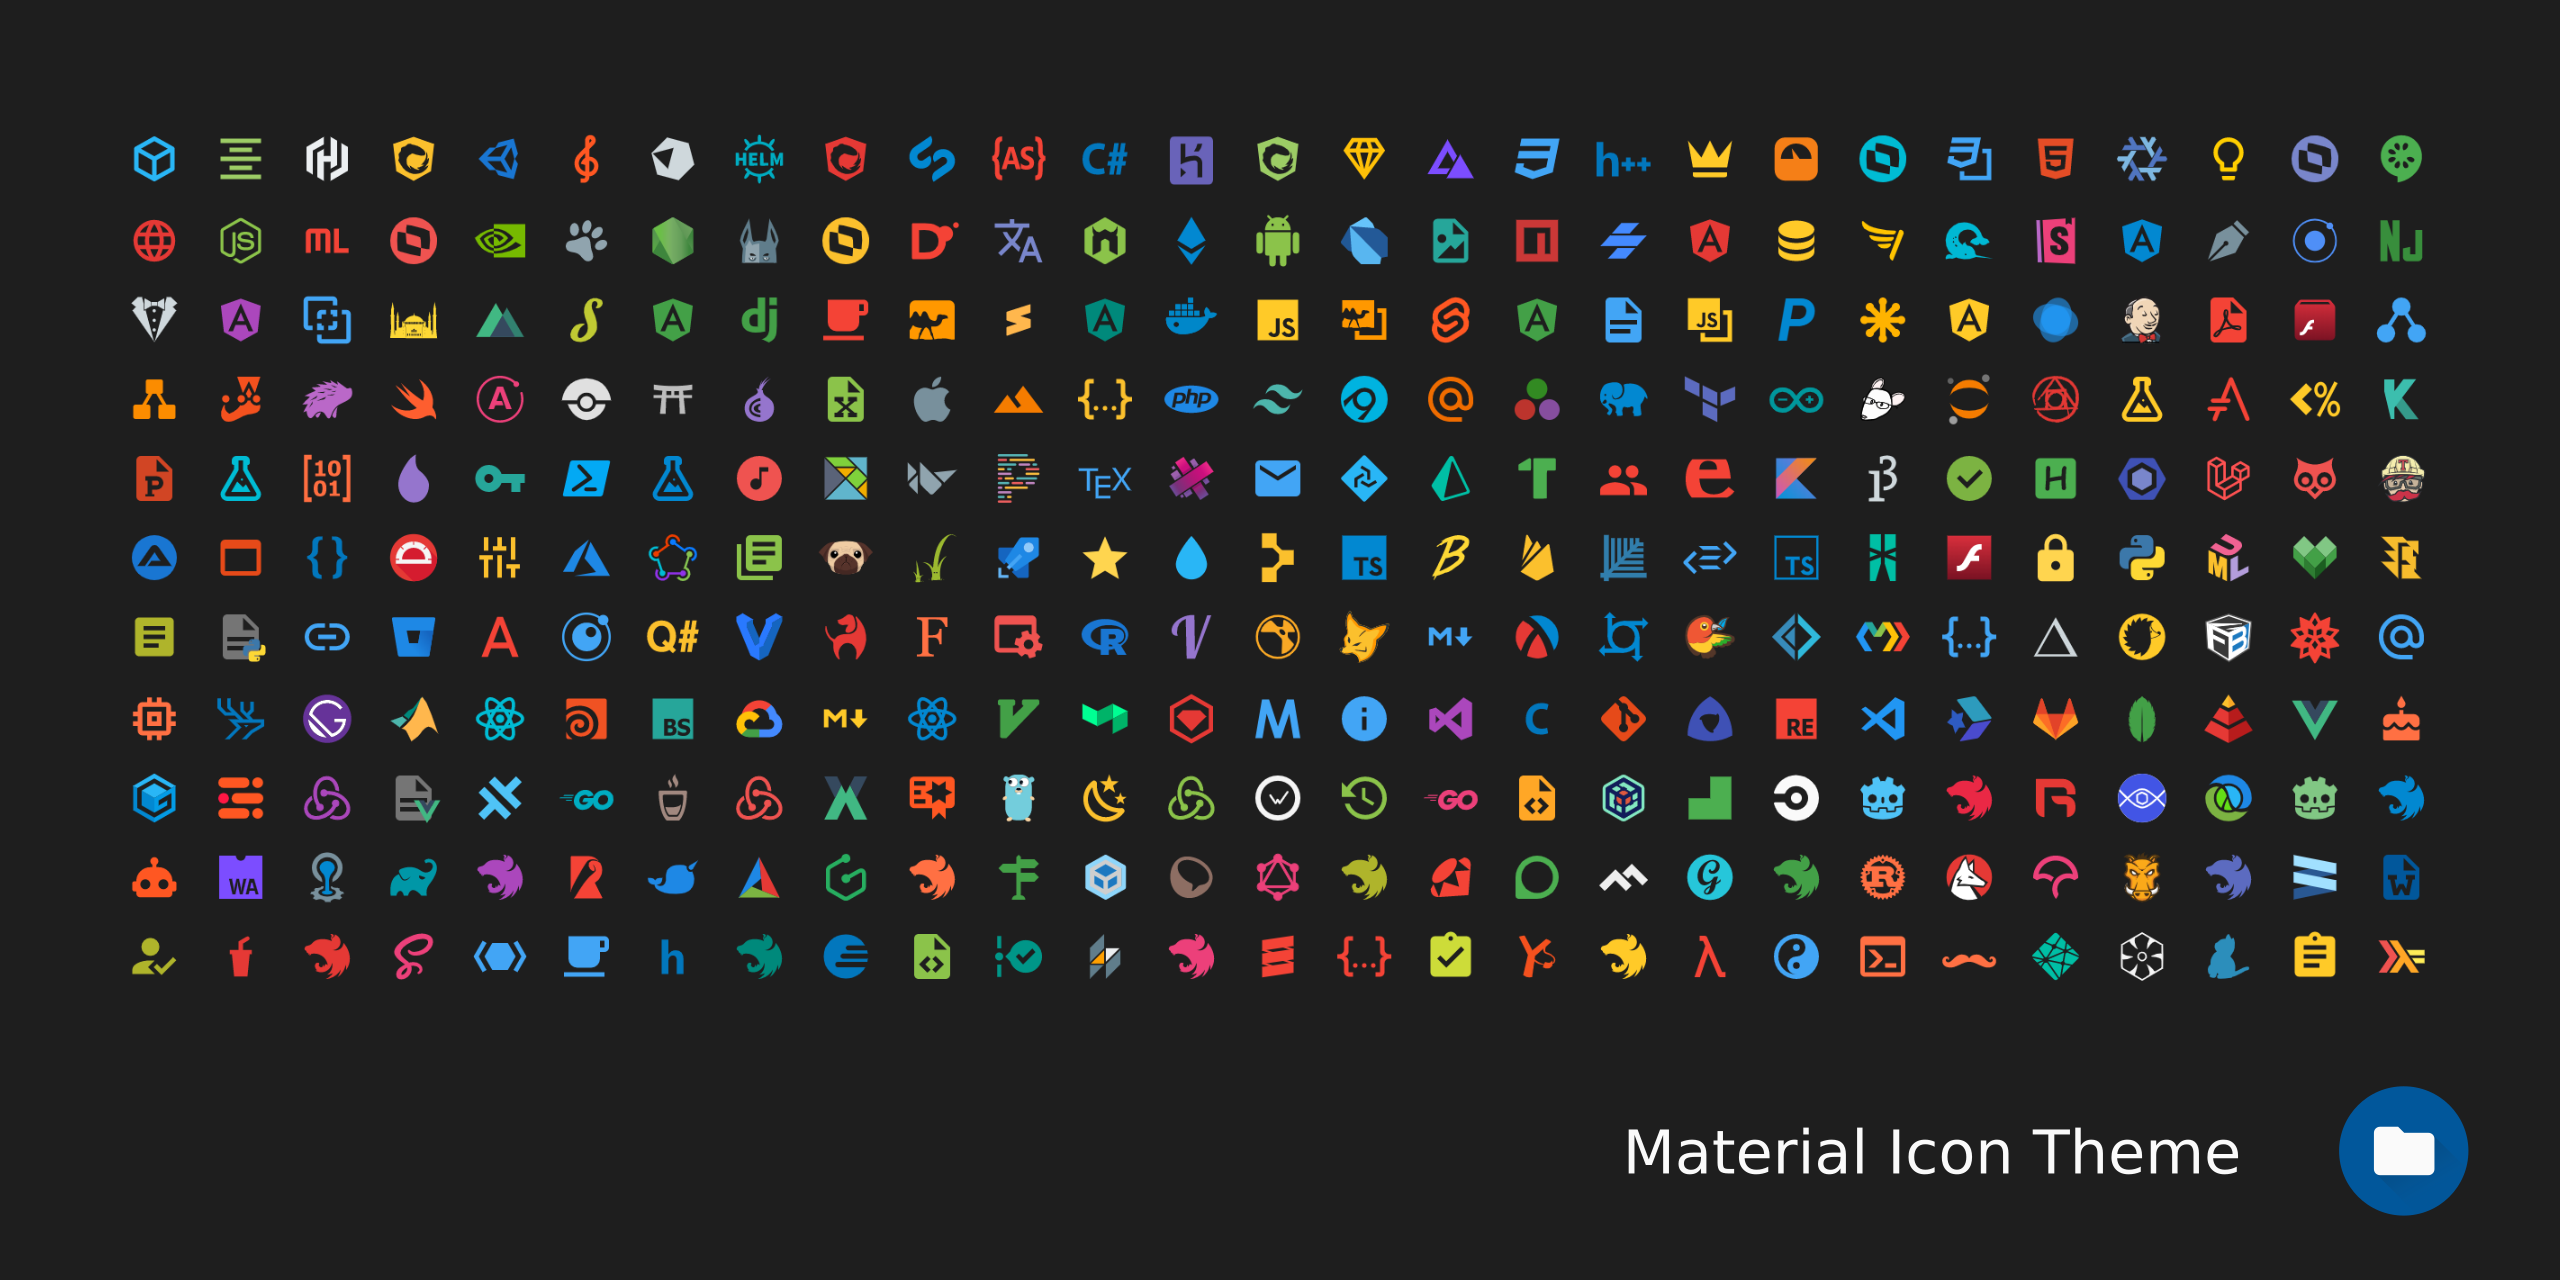
\includegraphics[width=13cm]{images/MaterialIcon.png}
  \caption{Material Icon Theme}
\end{center}
\end{figure}
\item
\textbf{Package Json Upgrade:} Mostra gli aggiornamenti disponibili in package.json. Offre azioni rapide per guidare nell'aggiornamento.
\end{itemize}

\section{Git}
\begin{figure}[h!]
\begin{center}
  
\includegraphics[width=4cm]{images/git_logo.jpg}
  \caption{Logo Git}
\end{center}
\end{figure}
Git è un software di controllo versione distribuito utilizzabile da interfaccia a riga di comando. \cite{GIT}\\
Un software di controllo versione è un'applicazione che permette di tenere traccia di tutti gli aggiornamenti apportati ad uno specifico progetto software, o "repository".\\
Oltre a mostrare una visione più generale e strutturata sul progetto, Git consente agli sviluppatori di implementare codice in team nella maniera più efficiente possibile cercando di ridurre i conflitti che possono nascere da uno sviluppo parallelo. Questo viene reso possibile grazie ad un sistema di branches, letteralmente rami, che permettono allo sviluppatore di lavorare in autonomia in una spazio completamente isolato dal resto del progetto. Per riunificare poi il nuovo codice implementato con il branch principale, lo sviluppatore potrà effettuare un'operazione di merge. \\
\begin{figure}[h!]
\begin{center}
  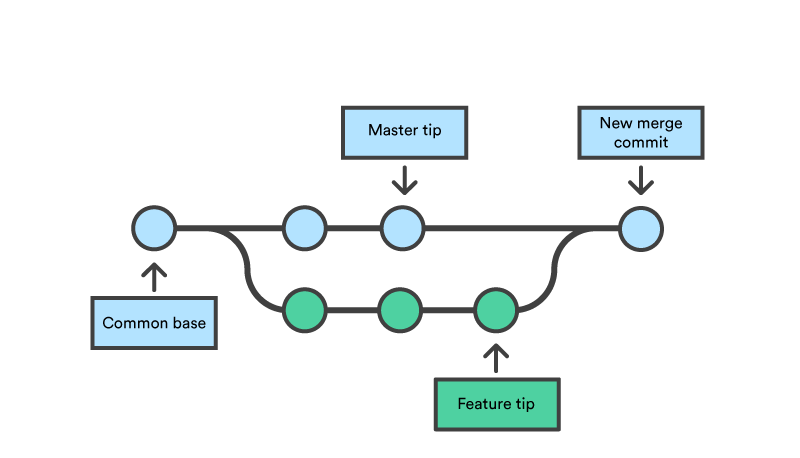
\includegraphics[width=12cm]{images/merge-di-due-branch.png}\\
  \caption{Esempio di merge di due branch in Git}
\end{center}
\end{figure}

\section{Gitlab}
\begin{figure}[h!]
\begin{center}
  
\includegraphics[width=7cm]{images/gitlab_logo.png}
  \caption{Logo GitLab}
\end{center}
\end{figure}
GitLab è una piattaforma web open source che permette la gestione di repository Git e di funzioni trouble ticket \cite{GITLAB}.\\
La piattaforma si basa sull'offrire uno spazio virtuale remoto, pubblico o privato, dove archiviare il proprio repository, permettendo agli sviluppatori di lavorare in team.
Inoltre GitLab consente di avere un controllo più immediato mettendo a disposizione dello sviluppatore una vista sui branch creati e una history delle modifiche apportate al repository. \\
Ulteriore funzionalità è quella dei trouble ticket, ovvero le "issues" all'interno di GitLab. Questo sistema consente di creare dei ticket per richiedere agli sviluppatori di aggiungere nuove funzionalità o di risolvere uno specifico bug. Una volta soddisfatta la richiesta il ticket potrà essere chiuso e disattivato dallo sviluppatore.
\begin{figure}[h!]
\begin{center}
  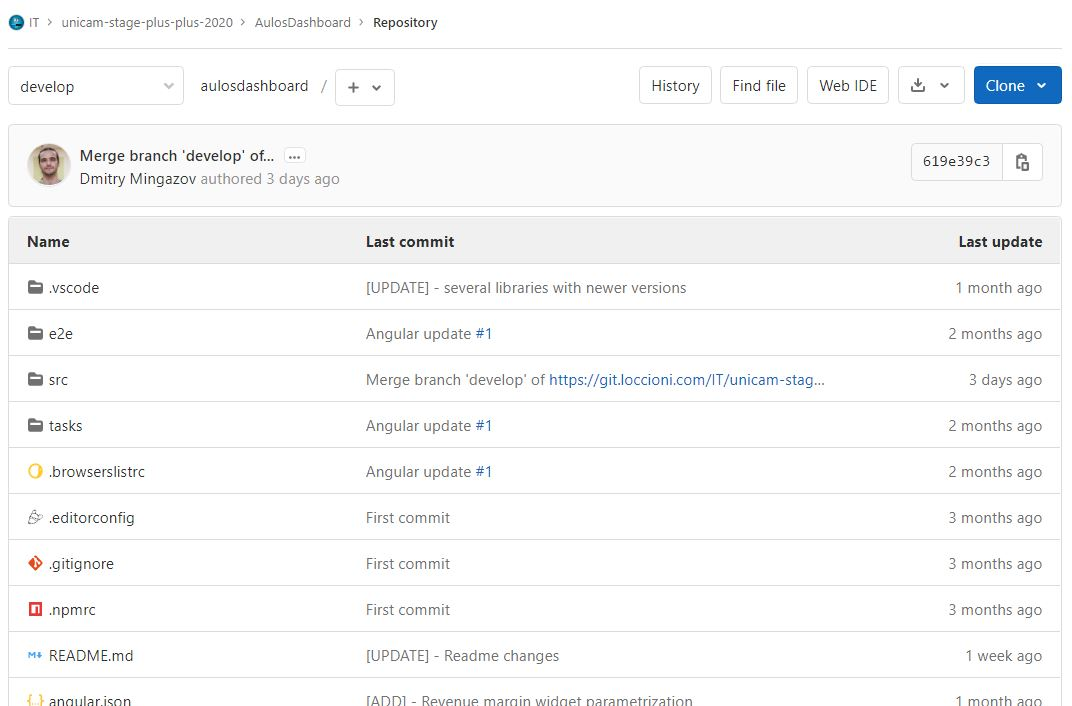
\includegraphics[width=13cm]{images/Repository_GitLab.JPG}
  \caption{Vista su una delle due repository caricate su GitLab}
\end{center}
\end{figure}
Il progetto discusso è stato archiviato su GitLab in un dominio privato Loccioni. 

\section{Postman}
\begin{figure}[h!]
\begin{center}
  
\includegraphics[width=4cm]{images/postman_logo.png}\\
  \caption{Logo Postman}
\end{center}
\end{figure}
Postman è uno strumento di sviluppo di API (application programming interface) che aiuta a costruire, testare e modificare API. Permette di fare vari tipi di richieste HTTP (GET, POST, PUT, PATCH), salvare gli ambienti per usi futuri e convertire le API in codice per vari linguaggi (come JavaScript, Python) \cite{POSTMAN}.\\
Nel corso dello sviluppo Postman è stato uno strumento essenziale per testare in modo veloce e immediato le richieste HTTP al backend.

\begin{figure}[h!]
\begin{center}
  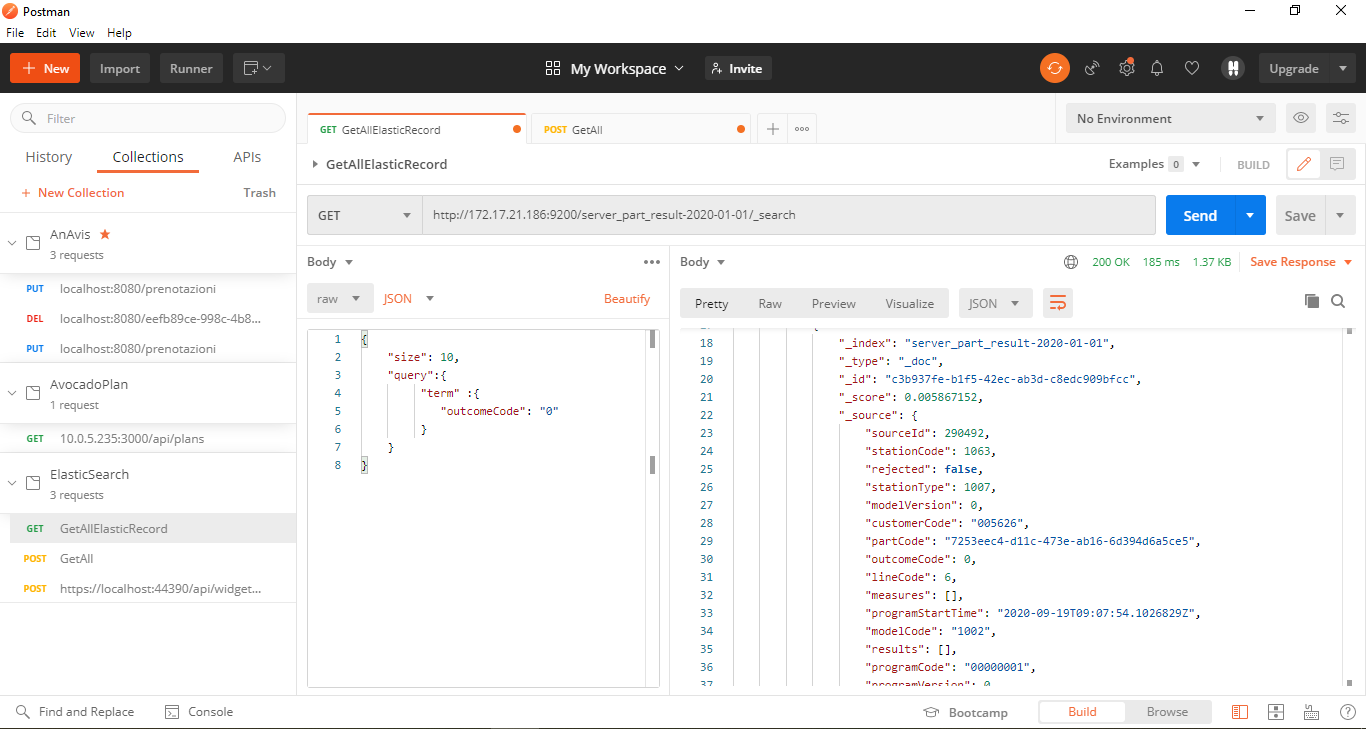
\includegraphics[width=15cm]{images/Postman.png}
  \caption{Schermata di Postman}
\end{center}
\end{figure}

\section{Angular 10}
\begin{figure}[h!]
\begin{center}
  
\includegraphics[width=7cm]{images/angular_logo.png}\\
  \caption{Logo Angular}
\end{center}
\end{figure}

L'applicativo frontend del progetto discusso nella tesi è stato sviluppato con Angular.\\
Angular è una piattaforma e un framework per costruire applicazioni client single-page usando i linguaggi HTML e TypeScript \cite{ANGULAR}. 
\paragraph{HTML} HTML (Hypertext Markup Language) è il linguaggio markup standard per i documenti visualizzabili in un browser web \cite{HTML}.
\paragraph{TypeScript} TypeScript è un linguaggio di programmazione open source sviluppato da Microsoft. Estende la sintassi di JavaScript, essendo un suo superset, in modo che qualunque programma scritto in JavaScript sia anche in grado di funzionare con TypeScript senza nessuna modifica. È stato progettato per lo sviluppo di grandi applicazioni ed è destinato a essere compilato in JavaScript per poter essere interpretato da qualunque web browser o app. \cite{TYPESCRIPT} \\
\\
L'architettura di un'applicazione Angular si basa su alcuni concetti fondamentali. Gli elementi costitutivi di base sono gli NgModules, che forniscono un contesto di compilazione per i Component. Questi ultimi sono elementi fondamentali per la costruzione delle UI in Angular. Ciascun Component definisce una classe che contiene dati e logica dell'applicazione ed è associato ad un modello HTML che definisce come verrà visualizzato nell'ambiente di destinazione. Il decoratore @Component() identifica la classe immediatamente sotto di essa come un componente e fornisce il modello e i relativi metadati specifici del componente.\\
I decoratori sono funzioni che modificano le classi JavaScript. Angular definisce un numero di decoratori che associano specifici tipi di metadati alle classi, in modo che il sistema sappia cosa significano quelle classi e come dovrebbero funzionare.\cite{ANGULAR} \\
\begin{lstlisting}[caption={Esempio di un Component in Angular}, style=javaScriptCode]
import { Component, OnInit } from '@angular/core';
@Component({
  selector: 'app-root',
  templateUrl: './app.component.html'
})
export class AppComponent implements OnInit {

  constructor() { }

  ngOnInit() { }
  
}
\end{lstlisting}
Per i dati o la logica che non sono associati a una vista specifica e che si desidera condividere tra i componenti, si crea una classe di servizio. Una definizione di classe di servizio è immediatamente preceduta dal decoratore @Injectable(). Il decoratore fornisce i metadati che consentono ad altri provider di essere inseriti come dipendenze nella tua classe.\\
La dependency injection (DI) consente di mantenere le classi dei componenti snelle ed efficienti. Non recuperano dati dal server, convalidano l'input dell'utente o accedono direttamente alla console; delegano tali compiti ai servizi \cite{ANGULAR} \\
\begin{lstlisting}[caption={Esempio di un Service in Angular}, style=javaScriptCode]
import { Injectable } from '@angular/core';
import { HttpClient } from '@angular/common/http';
import { Observable } from 'rxjs';
import { Data } from '...';

@Injectable({
  providedIn: 'root',
})
export class AppService {

  constructor( private http: HttpClient, private url: string ) { }
  
  public getData(): Observable<Data[]> {
    return this.http.get<Data[]>(this.url);
  }

}
\end{lstlisting}
Per la gestione interna dei pacchetti in Angular è stato utilizzato NPM (Node Package Manager). NPM è un gestore di pacchetti per il linguaggio di programmazione JavaScript. È il gestore di pacchetti predefinito per l'ambiente di runtime JavaScript Node.js. Consiste in un client da linea di comando, chiamato anch'esso npm, e un database online di pacchetti pubblici e privati, chiamato npm registry.
Il registry è accessibile via client e i pacchetti disponibili sono consultabili sul sito web di npm. \cite{NPM}

\section{KendoUI}
\begin{figure}[h!]
\begin{center}
  
\includegraphics[width=6cm]{images/kendo_logo.png}
  \caption{Logo Kendo UI}
\end{center}
\end{figure}
Kendo UI è un framework integrale di interfaccia utente HTML5 per costruire applicazioni e siti web interattivi e ad alte prestazioni. \cite{KENDO}
Il framework è stato usato all'interno dell'applicativo frontend con l'obiettivo di conferire un aspetto grafico più accattivante ai widget. Kendo UI per Angular offre un vasto numero di componenti:\\
\begin{figure}[h]
\begin{center}
  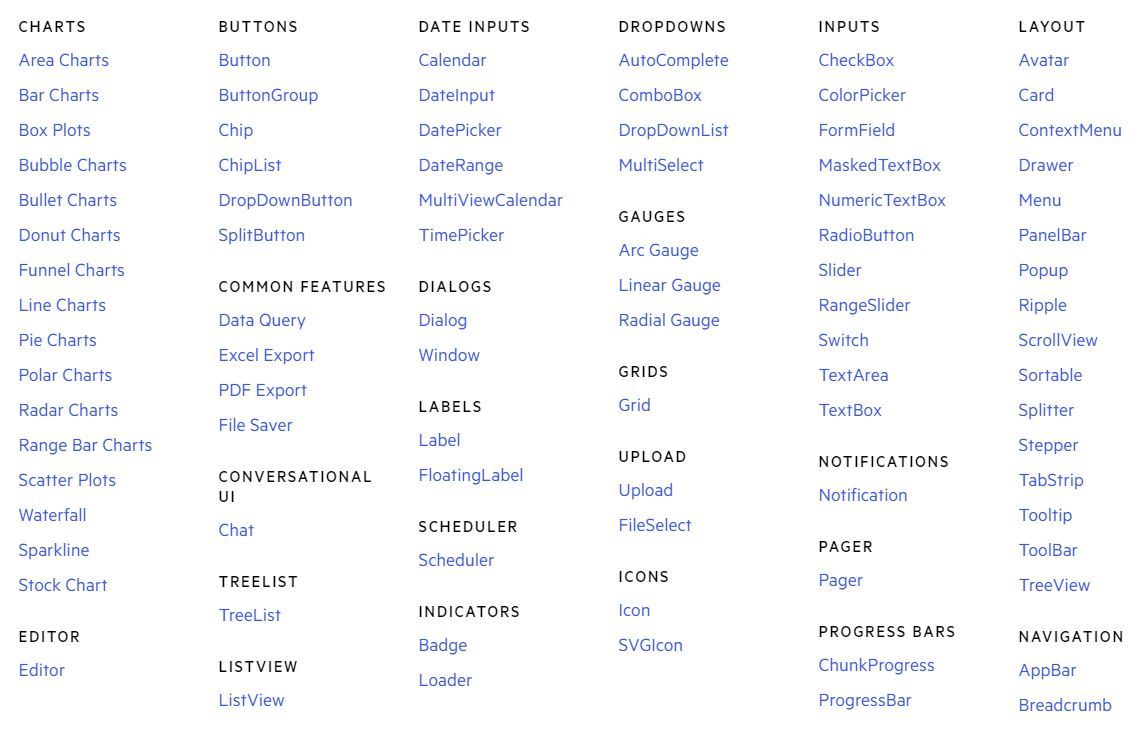
\includegraphics[width=15cm]{images/kendo_components.JPG}
  \caption{Componenti di Kendo UI per Angular}
\end{center}
\end{figure}
Ogni componente include un set completo di funzionalità già pronte all'uso \cite{KENDO}. Nel caso della Kendo Grid, componente frequentemente utilizzato nel progetto per rappresentare dei dati all'interno di una tabella, vi è ad esempio la possibilità di filtrare, ordinare, modificare e raggruppare i dati agevolmente. 
\begin{figure}[h!]
\begin{center}
  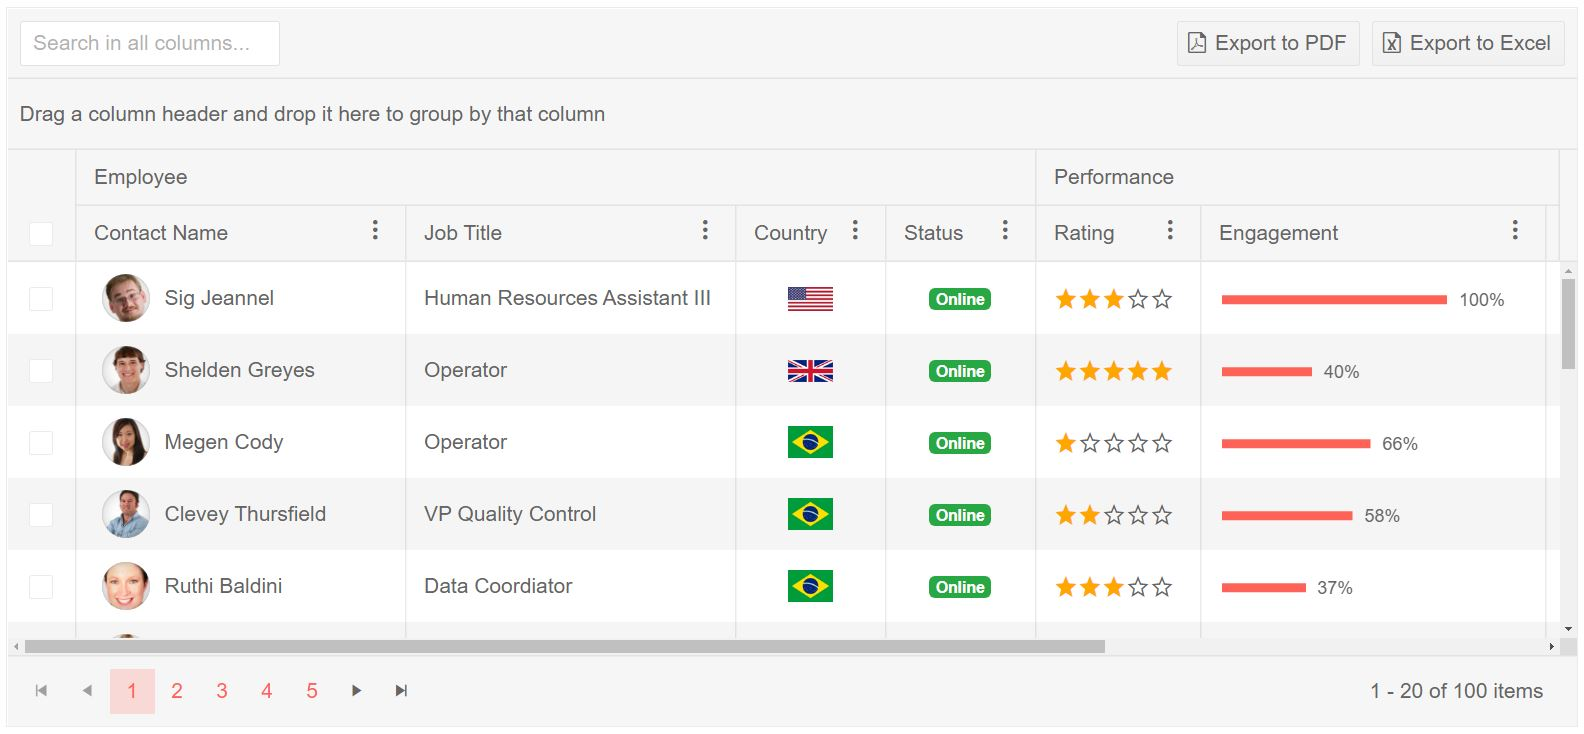
\includegraphics[width=14cm]{images/kendo_grid.JPG}
  \caption{Esempio di Kendo Grid per Angular}
\end{center}
\end{figure}

\section{JMeter}
\begin{figure}[h!]
\begin{center}
  
\includegraphics[width=6cm]{images/jmeter_logo.png}
  \caption{Logo JMeter}
\end{center}
\end{figure}
Apache JMeter™ è un software open source sviluppato interamente in Java e progettato per fare test di carico e misurare le prestazioni. Originariamente era stato pensato solamente per testare le applicazioni Web ma nel tempo sono state aggiunte altre funzionalità di testing. 
Può essere utilizzato per testare la resistenza di un server, una rete o un oggetto simulando diversi tipi di carichi pesanti per analizzarne le prestazioni complessive. \\
Le principali tipologie di applicazioni/server/protocolli che possono essere testate sono:
\begin{itemize}
    \item Web - HTTP, HTTPS (Java, NodeJS, PHP, ASP.NET, …)
    \item SOAP / REST Webservices
    \item FTP
    \item Database via JDBC
    \item LDAP
    \item Message-oriented middleware (MOM) via JMS
    \item Mail - SMTP(S), POP3(S) and IMAP(S)
    \item Native commands or shell scripts
    \item TCP
    \item Java Objects
\end{itemize}
\cite{JMETER} 
Apache JMeter è stato utilizzato per testare l'applicativo backend del progetto.

\section{HeidiSQL}
\begin{figure}[h!]
\begin{center}
  
\includegraphics[width=3cm]{images/HeidiSQL.png}
  \caption{Logo HeidiSQL}
\end{center}
\end{figure}
HeidiSQL è un software gratuito ed ha l'obiettivo di essere di facile comprensione, consente di visualizzare e modificare dati e strutture da computer che eseguono uno dei sistemi di database MariaDB, MySQL, Microsoft SQL, PostgreSQL e SQLite. Appartiene agli strumenti più popolari per MariaDB e MySQL in tutto il mondo \cite{HeidiSQL}. Tale strumento è stato utilizzato per la comunicazione con il server, al fine di manipolare le informazioni nei database che il server gestisce.

\section{Microsoft SQL Server Management Studio}
\begin{figure}[h!]
\begin{center}
  \includegraphics[width=5cm]{images/mssql.png}
  \caption{Logo MicrosoftSQL Server}
\end{center}
\end{figure}
SQL Server Management Studio (SSMS) è un ambiente gratuito ed integrato per la gestione di qualsiasi infrastruttura SQL, da SQL Server al database SQL di Azure. SSMS offre gli strumenti per configurare, monitorare e amministrare le istanze di SQL Server e i database. Usare SSMS per distribuire, monitorare e aggiornare i componenti del livello dati usati dalle applicazioni, nonché per creare query e script.
È possibile usare SSMS per eseguire query, progettare e gestire database e data warehouse in qualsiasi posizione, nel computer locale o nel cloud \cite{MSSQL}.

\pagebreak
\section{ElasticSearch}
\begin{figure}[h!]
\begin{center}
  
\includegraphics[width=6cm]{images/esearch.png}
  \caption{Logo ElasticSearch}
\end{center}
\end{figure}
Elasticsearch è un motore di ricerca e analisi full-text open source altamente scalabile. Consente di archiviare, cercare e analizzare grandi volumi di dati rapidamente e quasi in tempo reale. Viene generalmente utilizzato come motore sottostante per applicazioni che hanno caratteristiche e requisiti di ricerca complessi.
Elasticsearch dispone di diversi casi d'uso \cite{ELASTICSEARCH}:
\begin{itemize}
    \item consente di avere una visione più ampia delle informazioni a disposizione senza risultare dispersivo, anche con agglomerati di dati estremamente consistenti grazie alle "aggregazioni".
    \item combina diversi tipi di ricerche: strutturate, non strutturate, geografiche, ricerca di applicazioni, analisi della sicurezza, metriche e registrazione.
    \item si adatta a qualsiasi situazione che va dal semplice computer con un singolo nodo fino ad arrivare ad un cluster con centinaia di server, rendendo la creazione di un prototipo più agevole.
    \item utilizza API RESTful standard e JSON. L'apporto costante della comunità ha portato alla creazione e al mantenimento di client in molti linguaggi come Java, Python, .NET, SQL, Perl, PHP.
    \item è possibile utilizzare le funzionalità di ricerca e analisi in tempo reale di Elasticsearch per lavorare sui big data utilizzando il connettore Elasticsearch-Hadoop (ES-Hadoop).
\end{itemize}
Data l'elevata efficienza di questo software diverse compagnie informatiche l'hanno scelto per i loro prodotti. Gli ambiti interessati sono quelli di ricerca per quanto concerne Tinder, dove Elasticsearch permette di rendere il sistema più reattivo e veloce, mentre nel caso di Netflix l'utilizzo principale è focalizzato al giusto indirizzamento di notifiche push, email e messaggistica \cite{ELASTICSEARCH}.\\
Nel progetto discusso, Elasticsearch è stato utilizzato nell'implementazione del layer di accesso dei dati relativi alle macchine che testano le componenti degli elettrodomestici Whirlpool. In sinergia con questo strumento è stata impiegata la dashboard di visualizzazione dati Kibana.

\pagebreak
\section{Nest}
\begin{figure}[h!]
\begin{center}
  
\includegraphics[width=6cm]{images/elastic.png}
  \caption{Logo Nest}
\end{center}
\end{figure}
NEST è un client Elasticsearch .NET di alto livello che è ancora molto fedele all'API Elasticsearch originale. Tutte le richieste e le risposte sono esposte attraverso i tipi, rendendolo ideale per essere subito operativi.
Tutti i metodi disponibili all'interno di NEST sono esposti sia come versioni sincrone che asincrone, con quest'ultima che utilizza il suffisso idiomatico \verb|Async| sul nome del metodo \cite{Nest}.
Di seguito la medesima richiesta effettuata in Postman tramite un json ed in Nest.

figura~\ref{fig:hitratio} rappresenta la percentuale stimata di hit in cache durante il test, calcolata tramite la formula in fig.~\ref{fig:formula}.
\begin{figure}[h!]
     \centering
     \subfloat[Json body]{
         \centering
         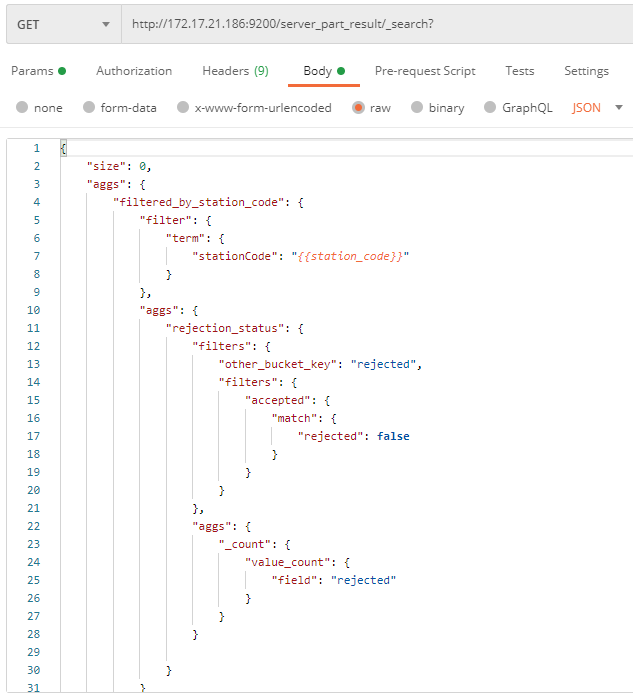
\includegraphics[width=12cm]{images/json.png}
         \label{fig:json}
         }
         \hfill
     \subfloat[Nest query]{
         \centering
         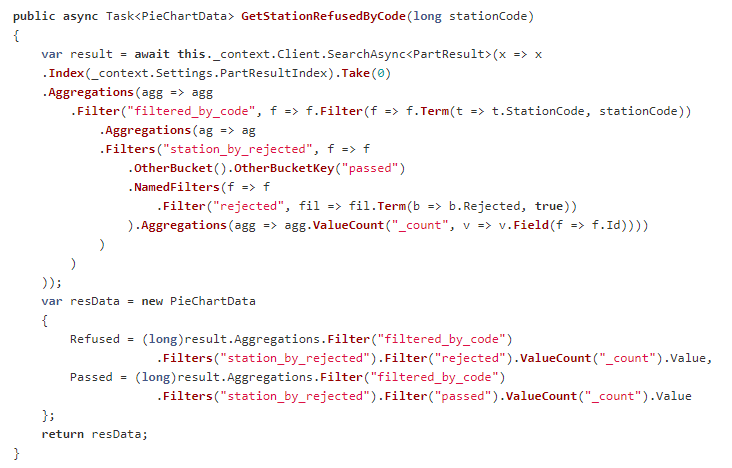
\includegraphics[width=15cm]{images/NestQuery.PNG}
         \label{fig:nest}
         }
        \caption{Stessa richiesta in json e Nest}
\end{figure}

\pagebreak
\section{Linq}
\begin{figure}[h!]
\begin{center}
  
\includegraphics[width=4.5cm]{images/linq.png}
  \caption{Logo Nest}
\end{center}
\end{figure}
LINQ (Language-Integrated Query) è il nome di un set di tecnologie basate sull'integrazione delle funzionalità di query direttamente nel linguaggio C\#. In genere, le query sui dati vengono espresse come stringhe semplici senza il controllo dei tipi in fase di compilazione o il supporto IntelliSense. È anche necessario imparare un linguaggio di query diverso per ogni tipo di origine dati: database SQL, documenti XML, svariati servizi Web e così via. Con LINQ, una query è un costrutto del linguaggio di prima classe, come le classi, i metodi e gli eventi. È possibile scrivere query su insiemi di oggetti fortemente tipizzati usando le parole chiave del linguaggio e gli operatori comuni. La famiglia di tecnologie LINQ offre coerenza per l'esecuzione di query per oggetti (LINQ to Objects), database relazionali (LINQ to SQL) e XML (LINQ to XML). Per uno sviluppatore che scrive query, la parte integrata nel linguaggio più visibile di LINQ è l'espressione di query. Le espressioni di query vengono scritte con una sintassi di query dichiarativa. Tramite la sintassi di query è possibile eseguire operazioni di filtro, ordinamento e raggruppamento sulle origini dati usando una quantità minima di codice \cite{Linq}.
\chapter{Architettura legacy}
%In questo capitolo verrà discussa la struttura precedentemente utilizzata %nell'applicativo e [...]
%L'applicativo presentava una parte backend che aveva la responsabilità di 
%fornire degli endpoint REST attraverso i quali l'applicativo frontend potesse %ottenere i dati da far visualizzare all'utente finale attraverso i widget
\section{Widget}
Un widget è una piccola applicazione, semplice e immediata, che mostra all'utente dati e informazioni, di solito sotto forma di grafici o tabelle.
La sua struttura si articolava in diversi file con scopi diversi:
\begin{itemize}
\item \textbf{widget.component.html} contiene il codice HTML che descrive l'aspetto grafico che il widget avrà all'interno della dashboard, e rappresenta i dati contenuti dal widget.component.ts
\item \textbf{widget.component.ts} è un Component Angular, contiene i dati che il widget deve visualizzare e si occupa di ottenere i dati interfacciandosi con il servizio opportuno
\item \textbf{widget.ts} è la classe che gestisce la configurazione del widget
\item \textbf{widget.service.ts} è un servizio Angular, contiene la logica di accesso ai dati che il widget deve visualizzare
\item \textbf{widget.module.ts} è un modulo Angular, contiene la dichiarazione del componente widget e la sua registazione al WidgetService
\end{itemize}

\subsection{Widget Component}
Il widget

\section{Struttura backend}
Lo sviluppo di un widget precedentemente si divideva nelle seguenti fasi:
\begin{itemize}
\item sviluppo del Widget Component
\item sviluppo di una classe Widget contenente la logica di business legata ai parametri
\item creazione di un modulo per il widget e conseguente registrazione in [...]
\item sviluppo di un servizio contenente la logica di ottenimento dati per il widget
\item sviluppo della logica di ottenimento dati nell'applicativo backend
\end{itemize}

%\chapter{Architettura}
In questo capitolo verrà esposta la struttura dell'applicativo e le differenze apportate al sistema precedentemente utilizzato, nonchè le procedure di scambio dati e configurazione del sistema.
\section{Widget}
\label{chap:widget}
\begin{figure}[h]
\centering
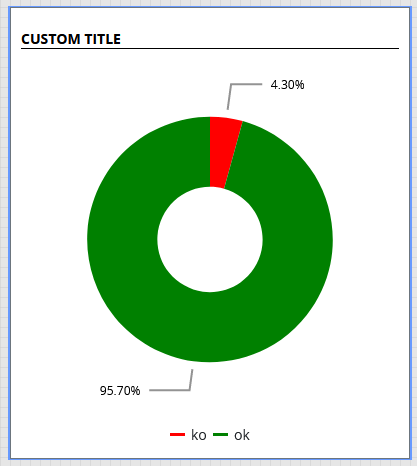
\includegraphics[scale=0.6]{images/widget_example.png}
\end{figure}
\subsection{Composizione}

Un widget è una piccola applicazione, semplice e immediata, che mostra all'utente dati e informazioni, di solito sotto forma di grafici o tabelle. \newline Prendendo ad esempio il pie chart widget si può vedere come un widget lato frontend sia formato da diversi file. La classe contenente i parametri volti alla visualizzazione grafica del widget si chiama \verb|PieChartWidget|. Estende la classe \verb|BaseWidget|, dove viene gestita tutta la logica per la presa dei dati dal backend, ed è decorata con il \verb|WidgetDecorator|, il quale aggiunge ulteriore comportamento al widget.



\begin{lstlisting}[caption={Classe PieChartWidget}, style=javaScriptCode]
@WidgetDecorator({
    endpoint: 'tuple',
    type: WidgetTypeEnum.MOBILITY,
    sourceable: true,
    adapter: PieChartAdapter,
    refreshableInfo: {
        refreshable: true,
    }
})
export class PieChartWidget extends BaseWidget {

    private titleParameter: StringParameter;

    constructor(injector: Injector, widgetDescriptor: WidgetDescriptor) {
        super(injector, widgetDescriptor);
        this.setSize(420, 450);
    }

    public get title(): string {
        return this.titleParameter.value;
    }

    protected createConfigParameters(): Observable<Parameter<unknown>[]> {
        this.createTitleParameter();
        return super.createConfigParameters();
    }

    private createTitleParameter() {
        this.titleParameter = new StringParameter('title', 'Title', 'My title');
        this.titleParameter.longText = 'Title Color';
        this.configParameters.push(this.titleParameter);
    }
}

\end{lstlisting}
Tutta la logica riguardante la visualizzazione dei dati del widget si trova nella classe \verb|PieChartComponent|. Al suo interno viene specificato come la label debba essere mostrata nel pie chart (con il metodo \verb|labelContent|) e viene implementato il metodo \verb|getDataCallback|, richiesto dalla classe \verb|BaseWidgetComponent| che viene estesa da \verb|PieChartComponent|, per salvarsi i dati ogni qualvolta il widget riceva dati dal backend.

\begin{lstlisting}[caption={Classe PieChartComponent}, style=javaScriptCode]
@Component({
    selector: 'app-pie-chart-widget',
    templateUrl: './pie-chart.component.html',
    encapsulation: ViewEncapsulation.None,
    changeDetection: ChangeDetectionStrategy.OnPush
})
export class PieChartComponent extends BaseWidgetComponent<PieChartWidget> {

    public data: TupleData[] = [];
    public backgroundColor = '#ffffff';

    constructor(widgetActions: WidgetActions, injector: Injector) {
        super(widgetActions, injector);
        this.labelContent = this.labelContent.bind(this);
    }

    public labelContent(args: LegendLabelsContentArgs): string {
        return `${args.dataItem.value.toFixed(2)}%`;
    }

    protected getDataCallback(value: any): void {
        this.data = value;
    }
}
\end{lstlisting}
Nel file HTML, di cui viene passato il path al @Component decorator, viene specificato l'aspetto grafico che avrà il widget all'interno della dashboard.

\begin{lstlisting}[caption={File pie-chart.component.html}, style=javaScriptCode]
<aulos-widget-layout [widget]="widget" [backgroundColor]="backgroundColor">
    <aulos-widget-title>
        {{ widget.title }}
    </aulos-widget-title>
    <aulos-widget-content>
        <kendo-chart #customChart [chartArea]="{opacity: 0}">
            <kendo-chart-legend position="bottom"></kendo-chart-legend>
            <kendo-chart-series>
                <kendo-chart-series-item type="donut" [data]="data" field="value" 
                        categoryField="label" colorField="color">
                    <kendo-chart-series-item-labels position="outsideEnd" color="#000" 
                            background="#FFFFFF" [content]="labelContent">
                    </kendo-chart-series-item-labels>
                </kendo-chart-series-item>
            </kendo-chart-series>
        </kendo-chart>
    </aulos-widget-content>
</aulos-widget-layout>
\end{lstlisting}
Infine ogni widget viene incluso in un modulo Angular. All'avvio dell'applicazione il widget viene registrato nel sistema con la chiamata del metodo \verb|registerWidgets|, presente nel modulo. Ciò permette ad AULOS di inserirlo nella lista di widget instanziabili nella dashboard.

\begin{lstlisting}[caption={Metodo all'interno del modulo che registra il widget nel sistema}, style=javaScriptCode]
private static registerWidgets(widgetsService: WidgetComponentsService): () => 
    Promise<any> {
        const result = (): Promise<any> => {
            return new Promise((resolve, reject) => {
                const myWidgetDescriptor: WidgetDescriptor = {
                    code: 'pieChartWidgetCode',
                    shortText: 'Pie Chart',
                    longText: 'Descrizione',
                    icon: 'fa fa-pie-chart',
                    group: 'Mobility Group'
                };
                widgetsService.register(myWidgetDescriptor, PieChartWidget, 
                    PieChartComponent);

                resolve();
            });
        };
        return result;
    }
\end{lstlisting}

\subsection{Le classi BaseWidget e BaseWidgetComponent}
Le classi \verb|BaseWidget| e \verb|BaseWidgetComponent| sono state create con l'obiettivo di alleggerire il carico di lavoro inerente allo sviluppo di un widget. In esse risiede tutta la logica di interfacciamento con il backend, lasciando come unica responsabilità alle classi che le estendono le modalità attraverso le quali vengono visualizzati i dati.
\\
\verb|BaseWidget| e \verb|BaseWidgetComponent| estendono rispettivamente le classi, già presenti nel framework AULOS, \verb|Widget| e \verb|WidgetComponent|.
\\
\paragraph{Base Widget}
Questa classe ha la responsabilità di ges
All'interno del \verb|BaseWidget| viene iniettato e utilizzato il \verb|WidgetService|, servizio in cui avvengono le chiamate REST, e vengono creati i parametri \verb|source| e \verb|filters|. 

\begin{lstlisting}[caption={Creazione dei parametri all'interno della classe BaseWidget}, style=javaScriptCode]
export class BaseWidget extends Widget {

    ...

    private createSourceParameter() {
        this.sourceParameter = new StringParameter('source', 'Source', '');
        this.sourceParameter.longText = 'Source';
        this.sourceParameter.descriptor.editor = new EditorDescriptor(EDITOR_BASE_PATH,
            'SourceEditor');
    }

    private createFiltersParameter() {
        this.filtersParameter = new ContainerParameter('filters', 'Filters', null);
        this.configParameters.push(this.filtersParameter);
    }

}
\end{lstlisting}

Il parametro \verb|source| indica da quale contesto verranno presi i dati da visuaizzare, mentre il parametro \verb|filters| contiene tutti i parametri che aggiungono filtri in fase di ottenimento dati (e.g. un intervallo di tempo per il quale si vogliono ottenere i risultati di un test). Il tutto viene inizializzato e caricato tramite il metodo \verb|initSourceCalls|.

\begin{lstlisting}[caption={Inizializzazione dei parametri all'interno della classe BaseWidget}, style=javaScriptCode]
export class BaseWidget extends Widget {
    
    ...
    
    private async initSourceCalls() {
        this.filtersParameter.stateChanges.subscribe(_ => {
            if (this.filtersSet && !this.widgetDTO) {
                this.getData();
            }
        });

        await this.sourceParameter.valueChanges.subscribe(sourceCode => {
            this.sourceSet = true;
            this.widgetService.getSourceProperties(sourceCode).subscribe
            (sourceProperties => {
                this.metadata = sourceProperties.metadata;
                this.setFilters(sourceProperties.filters);
                this.notifyStateChanged();
            });
        });
        this.initSource();
    }

    private getData() {
        if (!this.sourceParameter.value) { return; }
        if (!this.isFiltersReady()) { return; }
        this.widgetService.getData(this.endpoint, this.createRequest()).subscribe
            (value => {
                const data = MetadataService.map(value, this.metadata);
                this.widgetDataSubject.next(data);
        });
    }

    private initSource() {
        this.widgetService.getSource(this.endpoint).subscribe(sourceCode => {
            this.sourceParameter.value = sourceCode;
            this.sourceSet = true;
        });
    }

}
\end{lstlisting}
Nel \verb|BaseWidgetComponent| vi è la sottoscrizione al \verb|dataObservable|, attributo \verb|Observable| fornito da \verb|BaseWidget|, la quale si occupa di chiamare il metodo \verb|getDataCallback| ogni qualvolta vengono presi dati dal backend.
\begin{lstlisting}[caption={Metodi per l'inizializzazione dei dati all'interno della classe BaseWidgetComponent}, style=javaScriptCode]
@Directive()
export abstract class BaseWidgetComponent<T extends BaseWidget> extends 
    WidgetComponent<T> implements OnInit, OnDestroy{

    ...
        
    private initData() {
        this.widget.dataObservable.subscribe(value => {
            if (!value)
                {return;}
            this.getDataCallback(value);
            this.loading = false;
            this.changeDetectorRef.markForCheck();
        });
    }

    protected abstract getDataCallback(value: any): void;
}
\end{lstlisting}

\subsection{Il servizio WidgetService}
Nel \verb|WidgetService| avviene tutta la comunicazione tra frontend e backend.
La sua responsabilità è quella di fare chiamate REST per ottenere i dati da far visualizzare all'interno dei widget. Il principale metodo che si occupa di fare ciò è il metodo \verb|getData| in cui, passatagli una \verb|GenericRequest| composta da un sourceCode e un array di filtri, manda una richiesta POST al backend.

\begin{lstlisting}[caption={Metodo getData all'interno della classe WidgetService}, style=javaScriptCode]
@Injectable({
    providedIn: 'root'
})
export class WidgetService {

    ...

    public getData(widgetUrl: string, genericRequest: GenericRequest): 
        Observable<unknown[]> {
            const adapt = Adapters.getAdapter(widgetUrl);
            const restCall = this.http.post<unknown[]>(`${this.widgetsUrl}/${widgetUrl}`, 
            genericRequest);
            return adapt ? restCall.pipe(map((data) => adapt(data))) : restCall;
        }

}

\end{lstlisting}
Se esiste un'implementazione dell'\verb|Adapter|, interfaccia funzionale con il singolo metodo \verb|adapt|, per quel determinato widget, i dati che verranno presi saranno adattati prima di essere restituiti. In caso contrario verranno passati al widget dati grezzi.

La lista di sources disponibili e la possibile lista di filtri e metadati si ricavano rispettivamente dal metodo \verb|getSources| e dal metodo \verb|getSourceProperties|.

\begin{lstlisting}[caption={Metodi getSources e getSourceProperties all'interno della classe WidgetService}, style=javaScriptCode]
@Injectable({
    providedIn: 'root'
})
export class WidgetService {

    ...
        
    public getSources(widgetUrl: string): Observable<SourceInfo[]> {
        return this.http.get<SourceInfo[]>(`${this.apiUrl}/${widgetUrl}/discovery`);
    }

    public getSourceProperties(sourceCode: string): Observable<SourceProperties> {
        return this.http.get<SourceProperties>(`${this.apiUrl}/filters/${sourceCode}`);
    }

}
\end{lstlisting}
Se un widget è di tipo \verb|MOBILITY|, ovvero legato a dei dati provenienti dalle macchine Loccioni, avrà bisogno della possibilità di filtrare i dati in base alla linea, banco e stazione. Per questo all'interno del \verb|WidgetService| vi sono 3 metodi predisposti per il recupero di questi ultimi.

\begin{lstlisting}[caption={Metodi per recuperare linee, banchi e stazioni all'interno della classe WidgetService}, style=javaScriptCode]
@Injectable({
    providedIn: 'root'
})
export class WidgetService {

    ...
        
    public getLines(sourceCode: string): Observable<number[]> 
    {
        return this.http.get<number[]>(`${this.apiUrl}/topology/${sourceCode}
            /lines`);
    }

    public getBenches(sourceCode: string, lineCode: number): Observable<number[]> 
    {
        return this.http.get<number[]>(`${this.apiUrl}/topology/${sourceCode}
            /benches/${lineCode}`);
    }

    public getStations(sourceCode: string, stationCode: number): Observable<number[]> 
    {
        return this.http.get<number[]>(`${this.apiUrl}/topology/${sourceCode}
            /stations/${stationCode}`);
    }

}
\end{lstlisting}

\subsection{Il decorator factory WidgetDecorator}
Il \verb|WidgetDecorator| ha la responsabilità di aggiungere comportamento a un widget in base alle opzioni passate con l'interfaccia \verb|WidgetOptions|.

\verb|WidgetOptions| ha la seguente struttura:

\begin{lstlisting}[caption={Struttura delle WidgetOptions e delle RefreshableInfo}, style=javaScriptCode]
export interface WidgetOptions {
    // indicates which endpoint the widget has to use to take data from
    endpoint: string;
    // indicates the widget type (currently IT/MOBILITY)
    type: WidgetTypeEnum;
    // indicates whether or not the widget has a selectable source parameter
    sourceable?: boolean;
    /* indicates whether or not the widget has a refresh parameter and can be 
    used to set the default refresh rate*/
    refreshableInfo?: RefreshableInfo; 
    /* indicates the adapter class used to transform received data into a 
    more useful form*/
    adapter?: any;
}

export interface RefreshableInfo {
    refreshable: boolean;
    defaultRefreshRate?: RefreshRateEnum;
}
\end{lstlisting}
Il comportamento viene aggiunto al widget tramite altri decorators verificando le opzioni passate al momento della decorazione.

\begin{lstlisting}[caption={Decorator factory WidgetDecorator}, style=javaScriptCode]
export const WidgetDecorator: (options: WidgetOptions) => (target: Function) => 
    void = (options: WidgetOptions) => {

    return (target: Function) => {
        target.prototype.baseWidgetDecorator = true;
        target.prototype.endpoint = options.endpoint;

        switch (options.type) {
            case WidgetTypeEnum.IT:
                break;
            case WidgetTypeEnum.MOBILITY:
                Mobility(target);
                break;
        }
        if (options.sourceable) {
            Sourceable(target);
        }
        if (options.refreshableInfo?.refreshable) {
            Refreshable({defaultRefreshRate: options.refreshableInfo
                .defaultRefreshRate})(target);
        }

        if (options.adapter) {
            const adaptFunc = options.adapter.prototype.adapt;
            if (adaptFunc) {
                Adapters.setAdapter(target.prototype.endpoint, adaptFunc);
            }
        }
    };
};
\end{lstlisting}
\subsection{Mobility Decorator}
Il \verb|Mobility| decorator si occupa di aggiungere i parametri atti al filtraggio dei dati di un widget in base alla linea, banco e stazione.

\begin{lstlisting}[caption={Metodo di creazione dei parametri all'interno del decorator Mobility}, style=javaScriptCode]
export const Mobility: (target: Function) => void = (target: Function) => {

    ...

    target.prototype.createTopologyParameters = function(...args) {
        target.prototype.lineCodeParameter = new NumberParameter('lineCode', 
            'Line Code', 0);
        target.prototype.benchCodeParameter = new NumberParameter('benchCode', 
            'Bench Code', 0);
        target.prototype.stationCodeParameter = new NumberParameter('stationCode', 
            'Station Code', 0);

        this.lineCodeParameter.descriptor.editor = new EditorDescriptor(
            EDITOR_BASE_PATH, 'DropdownEditor', []);
        this.benchCodeParameter.descriptor.editor = new EditorDescriptor(
            EDITOR_BASE_PATH, 'DropdownEditor', []);
        this.stationCodeParameter.descriptor.editor = new EditorDescriptor(
            EDITOR_BASE_PATH, 'DropdownEditor', []);

        this.configParameters.push(this.lineCodeParameter);
        this.configParameters.push(this.benchCodeParameter);
        this.configParameters.push(this.stationCodeParameter);
    };

};
\end{lstlisting}
Il metodo che inizializza e definisce il comportamento che il widget avrà al cambio di uno dei parametri è il metodo \verb|initTopology|.

\begin{lstlisting}[caption={Metodo initTopology all'interno del decorator Mobility}, style=javaScriptCode]
export const Mobility: (target: Function) => void = (target: Function) => {

    ...

    target.prototype.initTopology = function(...args) {
        if (this.sourceSet) {
            this.getLines(this.sourceParameter.value, this);
        }
        this.sourceParameter.valueChanges.subscribe(sourceCode => {
            this.getLines(sourceCode, this);
        });

        this.lineCodeParameter.valueChanges.subscribe(lineCode => {
            this.resetBench(this);
            this.getData(this);
            if (this.sourceParameter.value) {
                this.widgetService.getBenches(this.sourceParameter.value, lineCode)
                    .subscribe(benchCodes => {
                    this.benchCodes = benchCodes;
                    this.benchCodeParameter.descriptor.editor.options = benchCodes;
                    this.benchCodeParameter.notifyStateChanged();
                });
            }
        });

        this.benchCodeParameter.valueChanges.subscribe(benchCode => {
            this.resetStation(this);
            this.getData(this);
            if (this.sourceParameter.value) {
                this.widgetService.getStations(this.sourceParameter.value, benchCode)
                    .subscribe(stationCodes => {
                    this.stationCodes = stationCodes;
                    this.stationCodeParameter.descriptor.editor.options = stationCodes;
                    this.stationCodeParameter.notifyStateChanged();
                });
            }
        });

        this.stationCodeParameter.valueChanges.subscribe(_ => {
            this.getData(this);
        });
    };

};
\end{lstlisting}

\subsection{Sourceable decorator}
Il \verb|Sourceable| decorator dà al widget la possiblità di far selezione all'utente la source dove prendere i dati dal backend.

Ogni widget che estende \verb|BaseWidget| ha al suo interno il parametro \verb|SourceParame|-\verb|ter|. Nel \verb|baseWidget| \verb|initSource| si occupa di impostare l'unica source da cui il widget prenderà i dati, mentre con l'override all'interno del \verb|Sourceable| decorator il metodo ha lo scopo di impostare la source in base a ciò che selezionerà l'utente.

\begin{lstlisting}[caption={Metodo initSource e override}, style=javaScriptCode]
export class BaseWidget extends Widget {
    
    ...
    
    private initSource() {
        this.widgetService.getSource(this.endpoint).subscribe(sourceCode => {
            this.sourceParameter.value = sourceCode;
            this.sourceSet = true;
        });
    }
    
}


export const Sourceable = (target: Function) => {

    ...

    target.prototype.initSource = function() {
        this.sourceParameter.valueChanges.subscribe(sourceCode => {
            this.sourceParameter.value = sourceCode;
        });
    };

};
\end{lstlisting}
La configurazione delle possibili source disponibili avviene nell'override del metodo \verb|initSourceCalls|. Le \verb|options| per l'\verb|editor| del \verb|sourceParameter| vengono impostate con il metodo \verb|setSources|.

\begin{lstlisting}[caption={Metodo setSources e override del metodo initSourceCalls all'interno del Sourceable Decorator}, style=javaScriptCode]
export const Sourceable = (target: Function) => {

    ...
    
    const oldInitSourceCalls = target.prototype.initSourceCalls;
    target.prototype.initSourceCalls = function() {
        this.widgetService.getSources(target.prototype.endpoint).subscribe(sources => {
            this.setSources(sources);
        });
        if (oldInitSourceCalls){
            oldInitSourceCalls.apply(this);
        }
    };

    target.prototype.setSources = function(sources: SourceInfo[]) {
        this.sourceParameter.descriptor.editor.options = sources;
    };

};
\end{lstlisting}
\subsection{Refreshable decorator}
Il \verb|Refreshable| decorator permette al widget di aggiornarsi e ricaricare i dati ad uno specifico intervallo di tempo. Il valore di default dell'intervallo può essere cambiato passando all'interno delle \verb|RefreshableInfo| anche un \verb|defaultRefreshRate|.
L'intervallo poi potrà essere selezionato dall'utente al momento di configurazione della dashboard grazie al \verb|refreshRateParameter| che viene aggiunto al widget.

\begin{lstlisting}[caption={Creazione del refreshRateParameter all'interno del Refreshable decorator}, style=javaScriptCode]
export const Refreshable: (options?: RefreshableOptions) => (Function) => 
    void = (options?: RefreshableOptions) => {
    return (target: Function) => {
        
        ...
        
        target.prototype.createRefreshParameter = function() {
            target.prototype.refreshRateParameter = new NumberParameter('refreshRate', 
                'Refresh Rate', this.defaultRefreshRate);
            this.refreshRateParameter.descriptor.editor = new EditorDescriptor(
                EDITOR_BASE_PATH,
                'EnumEditor',
                this.generateDefaultEnumOptions());
            this.configParameters.push(this.refreshRateParameter);
        };
        
    };
};
\end{lstlisting}
Ogni qualvolta un utente cambi intervallo di refresh viene effettuata una nuova registrazione all'Observable presente nel \verb|RefreshService|, legato a quel determinato intervallo, e viene annullata la precedente registrazione.

\begin{lstlisting}[caption={Metodo updateSubscription all'interno del Refreshable decorator}, style=javaScriptCode]
export const Refreshable: (options?: RefreshableOptions) => (Function) => 
    void = (options?: RefreshableOptions) => {
    return (target: Function) => {
        
        ...

        target.prototype.updateSubscription = function(refreshRate: number) {
            if (this.subscription) { this.subscription.unsubscribe(); }
            this.subscription = this.refreshService.getObservableOfInterval(refreshRate)
                .pipe(
                    exhaustMap(() => { this.getData(); return EMPTY; })
                )
                .subscribe();
        };
        
    };
};
\end{lstlisting}
Il \verb|RefreshService| ha la responsabilità di tenere salvati gli Observable legati a tutti gli intervalli richiesti.

\begin{lstlisting}[caption={Classe RefreshService}, style=javaScriptCode]
@Injectable({
  providedIn: 'root'
})
export class RefreshService {

  private intervals: Map<number, Observable<any>> = new Map();
  constructor() { }

  public getObservableOfInterval(refreshRate: number): Observable<any> {
    if (!this.intervals.has(refreshRate)) {
      this.intervals.set(refreshRate, interval(refreshRate).pipe(
        multicast(new Subject()),
        refCount()
      ));
    }
    return this.intervals.get(refreshRate);
  }
}
\end{lstlisting}
Nello specifico il metodo \verb|getObservableOfInterval| ritorna l'Observable dell'intervallo di tempo fornito. Se l'intervallo non è presente all'interno di \verb|intervals| allora lo inserisce creando l'Observable legato ad esso.

L'\verb|Observable| viene creato con il metodo \verb|interval|, il quale crea un \verb|Observable| che emette numeri sequenziali all'intervallo di tempo specificato. Poi viene trasformato con il metodo \verb|multicast| in un \verb|ConnectableObservable|, particolare tipo di \verb|Observable| che non emetterà valori finché non sarà chiamato il metodo \verb|connect|. Questa chiamata viene resa automatizzata grazie al metodo \verb|refCount|, il quale gestisce la connessione in modo tale da mantenerla attiva fintanto ci siano observer in ascolto.

\begin{lstlisting}[caption={Classe RefreshService}, style=html]
<aulos-editor-layout [editorConfiguration]="editorConfiguration">
  <ng-template aulosEditorSmallTemplate>
    <div class="input-group" [class.hidden]="disabled">
      <input type="text" 
        class="form-control form-control-sm is-invalid"
        [placeholder]=mySelection[0] ? mySelection[0] : 
        'Choose data source...'  | aulosTranslate 
        disabled readonly>
      <button class="btn btn-sm btn-icon" [disabled]="disabled" (click)="showExpandedModal()">
        <i class="fontaulos fontaulos-edit"></i>
      </button>
    </div>
  </ng-template>
  <ng-template aulosEditorCompactTemplate>
    <div class="input-group" [class.hidden]="disabled">
      <input 
      type="text" 
      class="form-control is-invalid" 
      [placeholder]="this.model.value ? 
      this.model.value : 
      'Choose data source...'  | aulosTranslate" 
      disabled
        readonly>
      <button class="btn btn-icon" [disabled]="disabled" (click)="showExpandedModal()">
        <i class="fontaulos fontaulos-edit"></i>
      </button>
    </div>
  </ng-template>
  <ng-template aulosEditorExpandedTemplate>
    <kendo-grid
              [data]="gridData"
              [style.maxlength]="501"
              [filterable]="true"
              [filter]="state.filter"
              [selectable]="selectableSettings"
              [sortable]="true"
              style="padding-top: 2%; padding-bottom: 5%;"
              (dataStateChange)="dataStateChange($event)"
              kendoGridSelectBy="sourceCode"
              [selectedKeys]="tmpSelection"
            >
            <kendo-grid-checkbox-column width="60%"></kendo-grid-checkbox-column>
            <kendo-grid-column field="sourceCode" filter="text"></kendo-grid-column>
            <kendo-grid-column field="shortText" filter="text"></kendo-grid-column>
            <kendo-grid-column field="longText" filter="text"></kendo-grid-column>
            <ng-template kendoGridNoRecordsTemplate>
              No sources available.
           </ng-template>
          </kendo-grid>
  </ng-template>
</aulos-editor-layout>
\end{lstlisting}
\chapter{Security}
\label{chap:security}

\paragraph{Module}
L'autenticazione degli utenti all'interno della dashboard è gestita dall' \verb|ItSecurity|-\verb|Module|. Nell'\verb|ItSecurityModule| vengono registrati nell'array \verb|providers|, che gestisce la dependency injection, i service necessari specificando per ognuno di essi la classe astratta a cui fanno riferimento e la classe d'implementazione.
\begin{lstlisting}[caption={Injection dei service nell'ItSecurityModule}, style=javaScriptCode]
@NgModule({
  imports: [HttpClientModule],
})
export class ItSecurityModule {
  /**
   * Main configuration to call on root application module
   */
  public static forRoot(): ModuleWithProviders<ItSecurityModule> {
    return {
      ngModule: ItSecurityModule,
      providers: [
        {
          provide: AbstractUserFactory,
          useClass: ItUserFactory
        },
        {
          provide: AbstractTokenProviderService,
          useClass: ItAccessTokenProviderService,
        },
        {
          provide: ItRefreshTokenProviderService,
          useClass: ItRefreshTokenProviderService,
        },
        {
          provide: AbstractSecurityService,
          useClass: ItSecurityService
        },
        {
          provide: HTTP_INTERCEPTORS,
          useClass: ITHttpSecurityInterceptor,
          multi: true
        },
        {
          provide: APP_INITIALIZER,
          useFactory: ItSecurityModule.appInitializer,
          deps: [AbstractTokenProviderService, ItRefreshTokenProviderService, 
            AbstractSecurityService],
          multi: true
        }
      ]
    };
  }
  ...
}
\end{lstlisting}
In \verb|providers| vengono fornite le implementazioni delle classi astratte
\verb|Abstract|-\verb|SecurityService|, \verb|AbstractUserFactory| e \verb|AbstractTokenProviderServi|-\verb|ce|, parte del framework Aulos.
Tutta la logica principale dell'autenticazione risiede all'interno dell'\verb|ItSecurityService|. La sua responsabilità è quella di autenticare e disconnettere l'utente nella dashboard. \\
\begin{lstlisting}[caption={Principali metodi della classe ItSecurityService}, style=javaScriptCode]
@Injectable({
  providedIn: 'root'
})
export class ItSecurityService extends AbstractSecurityService {

  ...

  login(username: string, password: string): Observable<ItUser> {
  
    ...
    
    return this.httpClient.post<JWTToken>(`${this.serviceConfiguration.baseUrl}/
    issue/oauth2/token`, { username, password, grant_type: 'password', 
        scope: 'urn:gl-services-infrastructure' }, { headers })
      .pipe(
        map(response => {
          const jwtUser = this.decodeToken(response.access_token);
          /* We have to set autologin to false to be sure to enable login phase 
          (when default user logout)*/
          this.serviceConfiguration.autoLogin = false;
          // Store current token so next call will have correct token
          this.accessTokenProviderService.store(btoa(JSON.stringify(jwtUser)));
          this.refreshTokenProviderService.store(response.refresh_token);
          this.currentJWTUser.next(jwtUser);
          return jwtUser;
        }),
        concatMap(jwtUser => {
          return this.getUser(jwtUser.loginName)
            .pipe(map(user => {
              this.currentUser.next(user);
              return user;
            }));
        }));
  }

  logout(): Observable<unknown> {
    this.accessTokenProviderService.remove();
    this.refreshTokenProviderService.remove();
    this.currentUser.next(null);
    return EMPTY;
  }

}
\end{lstlisting}
\paragraph{Grant}
Si è utilizzato il Resource Owner Password Credentials Grant \cite{GRANT} in quanto nel caso d'uso in questione si ha un elevato grado di fiducia tra frontend e backend.
Le credenziali vengono mandate all'Authorization Server che restituisce, se le credenziali sono corrette, un access token ed un refresh token.\\
\begin{figure}[h]
\begin{center}
\label{fig:grantflow}
\begin{verbatim}
+----------+
| Resource |
|  Owner   |
|          |
+----------+
     v
     |    Resource Owner
    (A) Password Credentials
     |
     v
+---------+                                  +---------------+
|         |>--(B)---- Resource Owner ------->|               |
|         |         Password Credentials     | Authorization |
| Client  |                                  |     Server    |
|         |<--(C)---- Access Token ---------<|               |
|         |    (w/ Optional Refresh Token)   |               |
+---------+                                  +---------------+

\end{verbatim}
\caption{Resource Owner Password Credentials Flow \cite{GRANT}}
\end{center}
\end{figure}
\FloatBarrier
\begin{figure}[h]
\begin{center}
\label{fig:refreshflow}
\begin{verbatim}
+--------+                                           +---------------+
|        |--(A)------- Authorization Grant --------->|               |
|        |                                           |               |
|        |<-(B)----------- Access Token -------------|               |
|        |               & Refresh Token             |               |
|        |                                           |               |
|        |                            +----------+   |               |
|        |--(C)---- Access Token ---->|          |   |               |
|        |                            |          |   |               |
|        |<-(D)- Protected Resource --| Resource |   | Authorization |
| Client |                            |  Server  |   |     Server    |
|        |--(E)---- Access Token ---->|          |   |               |
|        |                            |          |   |               |
|        |<-(F)- Invalid Token Error -|          |   |               |
|        |                            +----------+   |               |
|        |                                           |               |
|        |--(G)----------- Refresh Token ----------->|               |
|        |                                           |               |
|        |<-(H)----------- Access Token -------------|               |
+--------+           & Optional Refresh Token        +---------------+

\end{verbatim}
\caption{Token Refresh Flow \cite{REFRESH}}
\end{center}
\end{figure}
\FloatBarrier 
Il refresh token viene utilizzato dal Client per richiedere all'Authorization Server un nuovo access token quando quest'ultimo è scaduto.
La memorizzazione dell'access e del refresh token viene svolta rispettivamente dall'\verb|ItAccessTokenProviderService| e dall'\verb|ItRefreshTokenProviderService|.
Entrambe le classi estendono la classe astratta \verb|AbstractTokenProviderService|.\\
\begin{lstlisting}[caption={Classe astratta AbstractTokenProviderService}, style=javaScriptCode]
export declare abstract class AbstractTokenProviderService {
    /**
     * Get token from storage
     */
    abstract get(): Observable<string>;
    /**
     * Store token on storage
     */
    abstract store(token: string): Observable<void>;
    /**
     * Remove token on storage
     */
    abstract remove(): Observable<void>;
}
\end{lstlisting}
All'avvio della dashboard l'\verb|ItSecurityModule| autentica automaticamente l'utente se l'access token è già presente nel local storage.\newline
\begin{lstlisting}[caption={Login con token nell'ItSecurityModule}, style=javaScriptCode]
@NgModule({
  imports: [HttpClientModule],
})
export class ItSecurityModule {
    
  ...

  public static appInitializer(
    accessTokenProviderService: AbstractTokenProviderService,
    refreshTokenProviderService: ItRefreshTokenProviderService,
    securityService: AbstractSecurityService
  ): () => Promise<void> {
    const result = (): Promise<void> => {
      return new Promise((resolve, reject) => {
        // Check if token is already present on browser storage
        const sources = [accessTokenProviderService.get(), 
            refreshTokenProviderService.get()];
        forkJoin(sources).subscribe((val) => {
          const accTok: string = val[0];
          const refrTok: string = val[1];
          if (accTok && refrTok) {
            securityService.loginWithToken((JSON.parse(atob(accTok)) as ItJWTUser)
                .accessToken).subscribe(() => resolve());
          } else {
            resolve();
          }
        }, (error) => console.error(error));
      });
    };
    return result;
  }
}
\end{lstlisting}
\pagebreak
\paragraph{Interceptor} Chi intercetta e gestisce le richieste e le risposte http è l'\verb|ItHttpSecurityIntercep|-\verb|tor|.
Nello specifico l'\verb|ItHttpSecurityInterceptor| si occupa di: 
\begin{itemize}
    \item decorare le richieste http in uscita con token di autorizzazione, se l'header di autenticazione non è già presente nella richiesta,
    \item richiedere un access token tramite la procedura di refresh token in caso di risposta 401 a una richiesta al backend,
    \item ripetere la richiesta fallita con codice 401 dopo aver ottenuto il nuovo access token, 
    \item effettuare il logout in caso di fallimento della procedura di refresh.
\end{itemize}
\chapter{Parametri}

Un parametro, rappresentato dalla classe Parameter, rappresenta un valore con determinate caratteristiche che viene utilizzato in svariati contesti all'interno di AULOS.
\begin{lstlisting}[caption={Parameter.cs},style=sharpCode]
public class Parameter
{
    public Parameter();
    public string Code { get; set; }
    public ParameterDescriptor Descriptor { get; set; }
    public string Value { get; set; }
    public List<Parameter> SubParameters { get; set; }
    public string DescriptorCode { get; set; }
    public StandardParameterType Type { get; set; }
    public Parameter GetSubParameter(string code);
}
\end{lstlisting}
\begin{itemize}
\item Code è l'identificativo univoco del parametro
\item Descriptor è il descrittore del parametro, utilizzato per creare il parametro lato frontend
\item Value è il valore del parametro
\item SubParameters sono i sottoparametri del parametro (un parametro può rappresentare un'aggregazione di altri parametri)
\item Type rappresenta il tipo del valore rappresentato dal parametro
\end{itemize}
La classe ParameterDescriptor presenta
\begin{lstlisting}[caption={ParameterDescriptor.cs},style=sharpCode]
public class ParameterDescriptor
{
    public ParameterDescriptor();        
    public string Code { get; set; }
    public string ShortText { get; set; }
    public string LongText { get; set; }
    public StandardParameterType Type { get; set; }
    public string ContentType { get; set; }
    public ParameterEditor Editor { get; set; }
    public string MeasureUnit { get; set; }
    public string DefaultValue { get; set; }
    public string Format { get; set; }
    public ParameterValidator Validator { get; set; }
    public List<ParameterDescriptor> SubParameters { get; set; }
    public ParameterDescriptor ItemDescriptor { get; set; }
    public List<string> ItemDescriptorCodes { get; set; }
    public string WriteEnabledConditionCode { get; set; }
    public string VariantType { get; set; }
}
\end{lstlisting}
L'attributo Editor, istanza della classe ParameterEditor, descrive l'eventuale Editor utilizzato lato frontend per permettere la modifica del parametro da parte dell'utente

\section{Parameter Editor}
La classe ParameterEditor è così composta:
\begin{lstlisting}[caption={ParameterEditor.cs},style=sharpCode]
public class ParameterEditor
{
    public ParameterEditor();
    public string Type { get; set; }
    public string Path { get; set; }
    public dynamic Options { get; set; }
}
\end{lstlisting}
\begin{itemize}
\item Type è il codice univoco dell'Editor memorizzato lato frontend
\item Path è il path dove AULOS dovrà cercare l'editor
\item Options sono le eventuali opzioni che l'editor può avere
\end{itemize}

\subsection{Custom Editors}
AULOS fornisce diversi Editor per permettere all'utente di modificare i parametri, ma è possibile crearne di nuovi per casi d'uso più specifici. Un Editor è un Component Angular che va registrato all'interno dell'EditorFactory attraverso il metodo register .\\
\begin{lstlisting} [caption={dashboard-parameter-editors.module.ts},style=javascriptCode]
export class DashboardParameterEditorsModule {

    ...

    public static appInitializer(): () => Promise<void> {
        const result = (): Promise<void> => {
            return new Promise((resolve, reject) => {
            
                ...
                
                EditorFactory.register(
                    EDITOR_BASE_PATH,
                    'DropdownEditor',
                    DropdownEditorComponent);
                resolve();
            });
        };
        return result;
    }
}
\end{lstlisting}
Il template dell'Editor Component contiene tre direttive strutturali (aulosEditorSmallTemplate, aulosEditorCompactTemplate e aulosEditorExpandedTemplate) le quali contengono il codice html che deve essere visualizzato a seconda dello spazio in cui è contenuto l'Editor.
\begin{lstlisting}[caption={source-editor.component.html},style=html]
<aulos-editor-layout [editorConfiguration]="editorConfiguration">
  <ng-template aulosEditorSmallTemplate>
    <div class="input-group" [class.hidden]="disabled">
      <input type="text" 
        class="form-control form-control-sm is-invalid"
        [placeholder]="mySelection[0] ? 
        mySelection[0] : 
        'Choose data source...'  | aulosTranslate" 
        disabled readonly>
      <button class="btn btn-sm btn-icon" [disabled]="disabled" (click)="showExpandedModal()">
        <i class="fontaulos fontaulos-edit"></i>
      </button>
    </div>
  </ng-template>
  <ng-template aulosEditorCompactTemplate>
    <div class="input-group" [class.hidden]="disabled">
      <input 
      type="text" 
      class="form-control is-invalid" 
      [placeholder]="this.model.value ? 
      this.model.value : 
      'Choose data source...'  | aulosTranslate" 
      disabled
        readonly>
      <button class="btn btn-icon" [disabled]="disabled" (click)="showExpandedModal()">
        <i class="fontaulos fontaulos-edit"></i>
      </button>
    </div>
  </ng-template>
  <ng-template aulosEditorExpandedTemplate>
    <kendo-grid
              [data]="gridData"
              [style.maxlength]="501"
              [filterable]="true"
              [filter]="state.filter"
              [selectable]="selectableSettings"
              [sortable]="true"
              style="padding-top: 2%; padding-bottom: 5%;"
              (dataStateChange)="dataStateChange($event)"
              kendoGridSelectBy="sourceCode"
              [selectedKeys]="tmpSelection"
            >
            <kendo-grid-checkbox-column width="60%"></kendo-grid-checkbox-column>
            <kendo-grid-column field="sourceCode" filter="text"></kendo-grid-column>
            <kendo-grid-column field="shortText" filter="text"></kendo-grid-column>
            <kendo-grid-column field="longText" filter="text"></kendo-grid-column>
            <ng-template kendoGridNoRecordsTemplate>
              No sources available.
           </ng-template>
          </kendo-grid>
  </ng-template>
</aulos-editor-layout>
\end{lstlisting}
È necessario che l'Editor Component estenda BaseEditorComponent, classe che offre delle funzionalità di interfacciamento con AULOS, e che presenti la logica necessaria alla modifica del parametro a esso associato.

\section{Utilizzo dei parametri nell'applicativo}
Nell'applicativo, il parametro svolge una duplice funzione:
\begin{itemize}
\item permette di gestire la configurazione di un widget lato frontend
\item viene utilizzato per specificare dei filtri da applicare in fase di ottenimento dei dati
\end{itemize}
La classe Widget e le sue estensioni nell'applicazione frontend hanno la responsabilità di gestire i parametri legati ad un widget. Questi parametri possono rappresentare un attributo grafico del widget, un valore della sua configurazione oppure un filtro da applicare ai dati da visualizzare.
\begin{figure}[h!]
\begin{center}
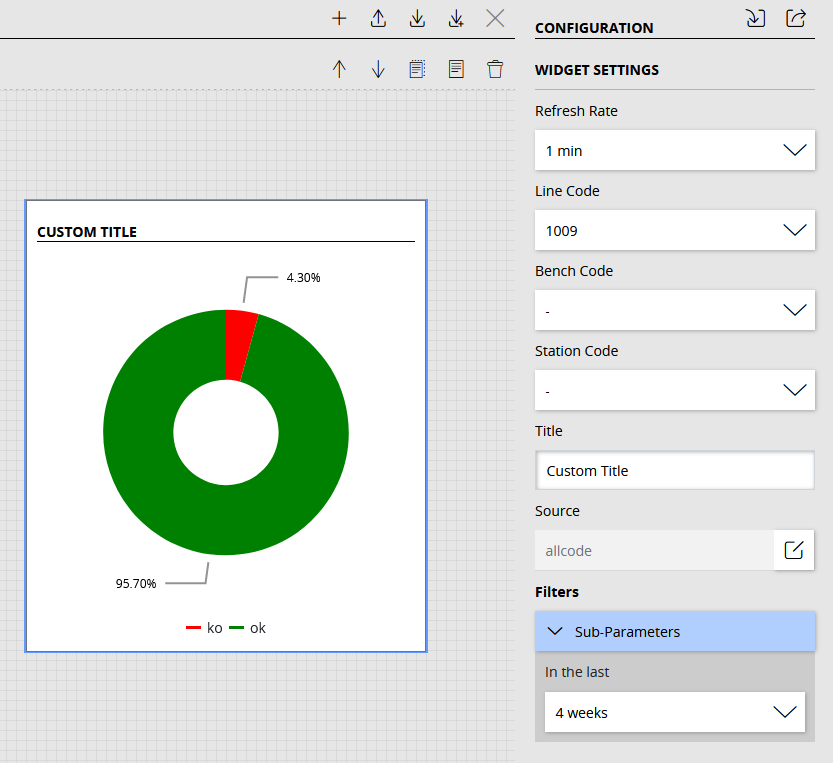
\includegraphics[scale=0.5]{parameters_example}\\
\caption{Possibile configurazione del widget PieChart}
\end{center}
\end{figure}
\subsection{Filter Parameters}
Data la capacità dei parametri di poter rappresentare dati eterogenei, sono stati utilizzati per rappresentare i possibili filtri di una query.\\
I Filter Parameters vengono generati attraverso dei ParameterDescriptor, presi con una chiamata REST (vedi Ch.~\ref{ch:sms}) dopo che è stata definita una source.
\begin{lstlisting}[caption={initSourceCalls, base-widget.ts},style=javascriptCode]
private async initSourceCalls() {

	...
	
        await this.sourceParameter.valueChanges.subscribe(sourceCode => {
            this.sourceSet = true;
            this.widgetService.getSourceProperties(sourceCode).subscribe(sourceProperties => {
                this.metadata = sourceProperties.metadata;
                this.setFilters(sourceProperties.filters);
                this.notifyStateChanged();
            });
        });
        this.initSource();
}
\end{lstlisting}
\section{Source Management}
\label{ch:sms}
Una source è un'astrazione che rappresenta una sorgente di dati visualizzabili da un widget. Ogni source viene identificata da una DataSource, una classe che nel pattern Model View Controller si colloca tra il Controller e il Model. La gestione delle source nel backend permette il riutilizzo di uno stesso widget per la visualizzazione di dati provenienti da contesti diversi.

\subsection{Creazione Source}
\label{sec:datasource}
Viene creata una classe DataSource che implementa l’interfaccia relativa al tipo di dato che deve ritornare. L'interfaccia presenterà un metodo volto ad ottenere i dati richiesti (e.g. GetData), che verrà implementato dalla DataSource.
\begin{lstlisting}[caption={ITupleDataSource.cs}, style=sharpCode]
interface ITupleDataSource
    {
        public TupleDTO[] GetData(List<Parameter> parameters);
    }
\end{lstlisting}
\begin{lstlisting}[caption={TupleDataSource.cs}, style=sharpCode]
public class AllRefusedDataSource : ITupleDataSource, ITopologyDataSource
{
  ...
  public TupleDTO[] GetData(List<Parameter> parameters)
  {
    var sam = new SeriousParameterHandler(parameters);
    var hours = sam.GetValue<long>("from");
    var now = DateTime.Now;
          DateTime from = now.AddHours(-hours);
    if (hours == -1)
          {
      from = new DateTime(0);
          }
    return sam.Contains("stationCode") ? 
      _repo.GetStationRefusedByCode(sam.GetValue<long>("stationCode"), from)
      .GetAwaiter().GetResult() :
      sam.Contains("benchCode") ? 
      _repo.GetBenchRefusedByCode(sam.GetValue<long>("benchCode"), from)
      .GetAwaiter().GetResult() :
      sam.Contains("lineCode") ?
      _repo.GetLineRefusedByCode(sam.GetValue<long>("lineCode"), from)
      .GetAwaiter().GetResult() :
              _repo.GetAllRefused(from)
      .GetAwaiter().GetResult();
  }
  ...
}
\end{lstlisting}

\subsection{Registrazione Source}
Le informazioni di una source sono descritte da SourceInfo e sono le seguenti:
\begin{itemize}
\item SourceCode è l’identificativo della source
\item TDataSource è il tipo della DataSource legata alla source
\item Parameters sono i parametri messi a disposizione dalla source per modificare la query
\item Metadata sono i metadati volti a modificare come vengono visualizzati i dati lato frontend
\end{itemize}
Parameters e Metadata vengono scritti in un file json all’interno della cartella \verb|properties| con il nome \verb|{SourceCode}.json|, come nel seguente esempio:
\begin{lstlisting}[caption={allcode.json}, style=JavaScriptCODE]
{
  "metadata": {
    "meta": {
      "fieldName": "label"
    },
    "properties": {
      "color": [
        {
          "field": "Passed",
          "value": "green"
        },
        {
          "field": "Refused",
          "value": "red"
        }
      ],
      ...
      ]
    }
  },
  "filters": [
    {
      "Code": "from",
      "ShortText": "In the last",
      "LongText": "From",
      "Type": "number",
      "DefaultValue": -1,
      "Editor": {
        "Type": "EnumEditor",
        "Path": "@aulos/parameter-editors",
        "Options": {
          "comboValues": [
            {
              "label": "12 hours",
              "value": 12
            },
            ...
            {
              "label": "Ever",
              "value": -1
            }
          ]
        }
      }
    }
  ]
} 
\end{lstlisting}
Per registrare una source, si crea una classe di configurazione che estende la classe astratta \verb|DiscoveryConfiguration|, e si richiama all’interno del costruttore il metodo \verb|AddSource|, passandogli le informazioni della source che si sta registrando.
\\
\begin{lstlisting}[caption={TupleDiscoveryConfiguration.cs}, style=sharpCode]
public class TupleDiscoveryConfiguration : DiscoveryConfiguration
{
    public TupleDiscoveryConfiguration()
    {
        AddSource(new SourceInfo
        {
            TDataSource = typeof(AllRefusedDataSource),
            SourceCode = "allcode",
            LongText = "All refused",
            ShortText = "All refused"
        });

        AddSource(new SourceInfo
        {
            TDataSource = typeof(RefusedTypeDataSource),
            SourceCode = "refusedtype",
            LongText = "Refused type",
            ShortText = "Refused type"
        });
    }
}
\end{lstlisting}
Il metodo AddSource, definito in DiscoveryConfiguration, ottiene attraverso PropertiesConfiguration le eventuali informazioni aggiuntive contenute nell’apposito file\\ \verb|{sourceCode}.json| per poi salvare la SourceInfo in una lista che verrà restituita attraverso il metodo pubblico Configure
\begin{lstlisting}[caption={DiscoveryConfiguration.cs}, style=sharpCode]
public abstract class DiscoveryConfiguration
{
    private List<SourceInfo> _sources = new List<SourceInfo>();
    public List<SourceInfo> Configure()
    {
        return _sources;
    }

    protected void AddSource(SourceInfo source)
    {
        var sourceProperties = PropertiesConfiguration.GetFilters(source.SourceCode);
        source.Parameters = sourceProperties.Filters.ToList();
        source.Metadata = sourceProperties.Metadata;
        _sources.Add(source);
    }

}
\end{lstlisting}
DataDiscoveryConfiguration ottiene tutte le classi che estendono DiscoveryConfiguration, per poi registrare in SourceManagementService tutte le source riscontrate
\begin{lstlisting}[caption={DataDiscoveryConfiguraton.cs}, style=sharpCode]
public static class DataDiscoveryConfiguration
{
  public static void Configure(SourceManagementService sourceManagementService)
  {
      var configurations = AppDomain.CurrentDomain.GetAssemblies()
          .SelectMany(x => x.GetTypes())
          .Where(x => typeof(DiscoveryConfiguration).IsAssignableFrom(x) && 
                  !x.IsInterface && !x.IsAbstract)
          .ToList();

      configurations.ForEach(configuration =>
      {
          sourceManagementService
              .RegisterSources(
                  ((DiscoveryConfiguration)Activator.CreateInstance(configuration))
                  .Configure()
              );
      });

  }
}
\end{lstlisting}
\subsection{Interazioni Frontend}
\label{chap:frontend}
DataTypeCoupling è un enum che associa ad ogni risorsa il tipo di DataSource che utilizza.
\begin{lstlisting}[caption={DataTypeCoupling.cs}, style=sharpCode]
...

public enum DataTypeCoupling
{
    [CouplingData(Label = "tuple", DataType = typeof(ITupleDataSource))]
    tupleData,
    [CouplingData(Label = "orders", DataType = typeof(OrdersDataSource))]
    ordersData,

    ... 

}
\end{lstlisting}
DiscoveryController presenta due endpoint:
\begin{itemize}
\item \verb|{resource}/discovery| - restituisce lo SourceCode e le descrizioni delle source associate ad una DataSource del tipo associato ad \verb|resource|, utilizzando il metodo GetDataSourcesByType di SourceManagementService
\item \verb|filters/{sourceCode}| - restituisce i parameters e i metadata di una specifica Source
\end{itemize}
Il sourceCode restituito durante questa fase verrà utilizzato dal frontend per richiedere i dati.

\subsection{Utilizzo}
Un Controller che restituisce dati in una determinata forma deve chiamarsi \verb|{resource}Controller|, dove resource è una stringa registrata in DataTypeCoupling.
\begin{lstlisting}[caption={TupleController.cs}, style=sharpCode]
 [Route("api/widgets/[controller]")]
 [ApiController]
 public class TupleController: ControllerBase
  {
  
  ...
  
  }
\end{lstlisting}
Deve presentare un endpoint Post nella forma \verb|api/widgets/{resource}|
\begin{lstlisting}[caption={TupleController.cs}, style=sharpCode]
[HttpPost]
public IActionResult Search([FromBody] GenericRequestDTO request)
{
    var dataSource = _sourceManagementService
      .GetDataSource<ITupleDataSource>(request.SourceCode);
    return new ObjectResult(dataSource.GetData(request.Filters));
}
\end{lstlisting}
Prende come Body una GenericRequest, che presenta i seguenti campi:
\begin{itemize}
\item \verb|SourceCode| indica da quale fonte di dati devono essere presi i dati.
\item \verb|Filters| sono gli eventuali parametri necessari alla esecuzione della query.
\end{itemize}
\begin{lstlisting}[caption={GenericRequestDTO.cs}, style=sharpCode]
public class GenericRequestDTO
{
    public string SourceCode { get; set; }
    public List<Parameter> Filters { get; set; }
}
\end{lstlisting}
Restituisce la risorsa gestita dal Controller utilizzando il metodo \verb|GetData| della DataSource che ottiene attraverso il metodo \verb|GetDataSource<T>| di \verb|SourceManagementService|, passandogli il SourceCode contenuto nella richiesta
\section{Topology}
\label{chap:topology}
I widget lato mobility sono impiegati per mostrare i dati provenienti dalle macchine la cui struttura si articola in: linee, banchi e stazioni; queste ultime sono la parte del macchinario volta ad effettuare i test sui vari componenti che attraversano la linea.

\subsection{ITopologyDataSource}
L'interfaccia \verb|ITopologyDataSource| contiene la definizione di tre metodi:
\\
\begin{lstlisting}[caption={TopologyController.cs}, style=javaScriptCode, label={lst:cacheattribute}]
    interface ITopologyDataSource
    {
        public List<int> GetLines();
        public List<int> GetBenches(int lineCode);
        public List<int> GetStations(int benchCode);
    }
\end{lstlisting}
Le classi che attualmente la implementano sono \verb|AllRefusedDataSource| e\\ \verb|RefusedTypeDataSource|, le quali andranno a richiamare i metodi necessari per la richiesta della lista dei codici di linee, banchi o stazioni, presente nella repository collegata ad un database MySQL.

\subsection{Controller Topology}
Quando si procede con la creazione di un widget mobility è possibile scegliere la source, in modo tale da definire la fonte in cui reperire i dati da visualizzare. In seguito,  facendo riferimento al formato standard dei macchinari, si ha la possibilità di scegliere il codice della linea, del banco e della stazione di cui si vogliono osservare i risultati.
Per poter scegliere questi codici vengono effettuate tre diverse chiamate al backend, in cui il controller definisce tre richieste \verb|HttpGet|: \\
\begin{lstlisting}[caption={TopologyController.cs}, style=javaScriptCode, label={lst:cacheattribute}]
        [HttpGet("{sourceCode}/lines")]
        public IActionResult GetLines([FromRoute] string sourceCode)
        {
           var dataSource = _sourceManagementService
           .GetDataSource<ITopologyDataSource>(sourceCode);
            return new ObjectResult(dataSource.GetLines());
        }

        [HttpGet("{sourceCode}/benches/{lineCode}")]
        public IActionResult GetBenches([FromRoute] string sourceCode, int lineCode)
        {
            var dataSource = _sourceManagementService
            .GetDataSource<ITopologyDataSource>(sourceCode);
            return new ObjectResult(dataSource.GetBenches(lineCode));
        }

        [HttpGet("{sourceCode}/stations/{benchCode}")]
        public IActionResult GetStations([FromRoute] string sourceCode, int benchCode)
        {
            var dataSource = _sourceManagementService
            .GetDataSource<ITopologyDataSource>(sourceCode);
            return new ObjectResult(dataSource.GetStations(benchCode));
        }
\end{lstlisting}
Tramite il metodo \verb|GetDataSource<DataSource>| definito in \verb|SourceManagemetService|, viene creata l'istanza della DataSource che implementa \verb|ITopologyDataSource|, in base al code passato come parametro.\\
Fornendo questa interfaccia come tipo, si ha la certezza che siano stati implementati i metodi volti al reperimento delle liste di codici di linee, banchi e stazioni.
\section{Persistence}
\label{chap:persistence}
Il Persistence Layer, in letteratura \textit{Data Access Layer}, è utilizzato per la manipolazione dei dati archiviati in una memoria persistente.\\
La corrispondenza tra modello object oriented (\textit{domain model}) e schema del database è data in gestione ad un framework \textit{ORM} (Object-Relational Mapping) \cite{EF}: Entity Framework, il quale ha la funzione di semplificare le operazioni di interrogazione e manipolazione dei dati.

\subsection{Struttura Persistence}
\begin{figure}[h!]
\begin{center}
  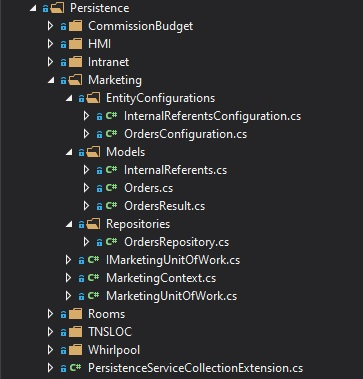
\includegraphics[width=8cm]{images/Persistence.jpg}\\
  \caption{Formato cartella persistence}\label{fig:persistence}
\end{center}
\end{figure}

Nella conformazione che si denota in figura~\ref{fig:persistence}, ciascuna cartella definisce un contesto applicativo ed è articolata in:

\begin{itemize}
\item 
\textbf{Entity configurations:} vi sono le configurazioni delle entità presenti in \textbf{Models} e vi si effettua il \textit{mapping} di tabelle e colonne nel database.
\item
\textbf{Models:} ciascun modello è un'entità che rappresenta l'analogo del record, o riga, di una tabella.
\item 
\textbf{Repositories:} volte all'interrogazione e manipolazione dati tramite l'uso di \textit{Data Manipulation Language} (quali Linq e Nest, rispettivamente per database SQL ed ElasticSearch).
\item 
\textbf{IUnitOfWork:} interfaccia in cui vengono definite \textit{repository} e metodo \verb|SaveChanges|.
\item
\textbf{DbContext:} in questa classe viene fornita la \textit{connection string} del database (definita in \verb|appsettings|), si dichiarano i DbSet relativi ai model, che sono entity set utilizzati per le \textit{CRUD operation} \cite{DbSet} e in \verb|OnModelCreating| si applicano le configurazioni dei model.
\item 
\textbf{UnitOfWork:} implementa l'interfaccia creando la repository e applicando il metodo \verb|SaveChanges| al context; quest'ultimo ha la funzione di salvare un insieme di modifiche in una transazione, oppure di eseguire un \textbf{rollback} (ossia un ripristino allo stato che precede l'aggiornamento).
\end{itemize}
\verb|PersistenceServiceCollectionExtension| si occupa di configurare le \textit{dependency injection} per la creazione del context ElasticSearch.
\section{Caching}
\label{ch:caching}
Il caso d'uso del progetto in questione prevede una moltitudine di dashboard collegate simultaneamente a un solo backend; al fine di  migliorare la performance è stato applicato un alleggerimento del carico tramite un \textit{middleware} \footnote{Il middleware è un software assemblato nella pipeline di app per gestire richieste e risposte. \cite{Middleware}} ASP.NET di cache. Ciò ha permesso la riduzione delle richieste effettivamente soddisfatte con dati generati appositamente da database SQL ed ElasticSearch sottostanti.
\subsection{Implementazione}
Il sistema di cache è stato implementato basandosi su un'implementazione già esistente di \textit{IMemoryCache} in ASP.NET Core. \cite{MemCache}
\begin{lstlisting}[caption={Startup.cs, iniezione Memory Cache}, style=javaScriptCode]
services.AddMemoryCache(options => Configuration.Bind("Cache", options));
\end{lstlisting}

La chiave di cache viene generata dal frontend nell'interceptor HTTP come \textit{hash} MD5 \cite{MD5} della concatenazione tra metodo \cite{HTTPMETHODS}, url con parametri \cite{HTTPPARAMS} e corpo \cite{HTTPBODY} della richiesta HTTP in uscita.
\begin{lstlisting}[caption={it-http-security.interceptor.ts, riga 28}, style=javaScriptCode]
mergeMap(token => {
          this.md5.appendAsciiStr(request.method).appendAsciiStr(request.urlWithParams)
          .appendStr(JSON.stringify(request.body));
          request = request.clone({
            setHeaders: {
              Authorization: `Bearer ${token}`,
              'AULOS-hash': this.md5.end(false) as string
            }
          });
          return next.handle(request).pipe(catchError(error => {
            if (error instanceof HttpErrorResponse && error.status === 401) {
              return this.handle401Error(request, next);
            } else {
              return throwError(error);
            }
          
\end{lstlisting}

Il middleware di cache controlla se la richiesta in arrivo ha header \textit{AULOS-hash} e, se esistente, controlla se ha già una \textit{entry in cache} associata. In caso positivo, il middleware non chiama il middleware successivo nella catena e restituisce la entry salvata.
\begin{lstlisting}[caption={TotallyOriginalCachingMiddleware.cs, Cache hit}, style=javaScriptCode]
context.Request.Headers.TryGetValue("AULOS-hash", out StringValues key);
            if (_cache.TryGetValue(key, out CustomCacheEntry entry))
            {
                await WriteResponse(context, entry);
                return;
            }
\end{lstlisting}

Per permettere allo sviluppatore backend di decidere a quali richieste limitare l'inserimento in cache, è stato implementato un attributo di cache estensione di \\ \textit{ActionFilterAttribute} \cite{ACTIONFILTER}, che, se anteposto a un controller o a un metodo HTTP di un controller, permette di decorare il contesto della relativa richiesta HTTP \cite{HTTPCONTEXT} in arrivo con flag \textit{ServerDuration} necessario a distinguere richieste abilitate all'inserimento in cache.
Il flag contiene la durata delle entry di cache relative all'azione a cui è applicato l'attributo di cache.

\begin{lstlisting}[caption={CacheAttribute.cs}, style=javaScriptCode, label={lst:cacheattribute}]

    public class CacheAttribute : ActionFilterAttribute
    {
        public int ServerDuration { get; set; }
        public override void OnActionExecuting(ActionExecutingContext context)
        {
            if (ServerDuration > 0)
            {
                context.HttpContext.Items["ServerDuration"] = $"{ServerDuration}";
            }
            else context.HttpContext.Items.Add("ServerDuration", 120);
            base.OnActionExecuting(context);
        }
    }
\end{lstlisting}

In caso negativo, il middleware lascia procedere la \textit{pipeline} e, se è presente nel contesto HTTP \cite{HTTPCONTEXT} il flag \textit{ServerDuration} generato da attributi di cache \cite{ACTIONFILTER} (Fig.~\ref{lst:cacheattribute}), salva la risposta generata dalla pipeline come entry in cache di durata \textit{ServerDuration} e lascia procedere la pipeline. Se non sono presenti flag, il middleware lascia procedere la pipeline senza effettuare azioni.

\begin{lstlisting}[caption={TotallyOriginalCachingMiddleware.cs, Cache miss}, style=javaScriptCode]
entry = await CaptureResponse(context);

       if (IsNotServerCachable(context))
           return;
       if (entry != null)
       {
           int serverCacheDuration = int.Parse((string)context.Items["ServerDuration"]);

           _cache.Set(key, entry, TimeSpan.FromSeconds(serverCacheDuration));
           }
       }
\end{lstlisting}

\chapter{Load Testing}
\label{ch:stresstesting}
Si è testata la capacità del sistema di offrire funzionalità senza interruzioni all'aumentare del carico. 
Si è optato per effettuare\textit{ load test} su backend tramite una \textit{suite di test} JMeter. \cite{JMETER}

\section{Implementazione}

I test sono stati impostati per effettuare automaticamente la procedura di login per poi usare \textit{l'access token} così ottenuto per autenticare le richieste inviate verso il backend.

Sono stati simulati 250 utenti concorrenti emettenti richieste a endpoint che prevedono l'uso di \textit{cache}, ripetendo test con lifetime variabili delle \textit{entry} in cache.
La dimensione della tabella di cache è stata mantenuta costante (60000 entry) generando casualmente valori di header \verb|AULOS-hash| (Ch. \ref{ch:caching}).
Il corpo delle richieste è stato fornito tramite un file .csv contenente tutte le possibili richieste generabili da un utente tramite la dashboard.

Testando la performance del backend quando sottoposto a un carico molto superiore a quello previsto dal caso d'uso dell'applicativo, è possibile avere un certo grado di sicurezza che il sistema sarà stabile una volta in utilizzo.

\section{Risultati}
Sono stati eseguiti test senza cache e con \textit{lifetime} di entry in cache pari a 5, 15, 30 e 120 secondi. 
Una volta eseguiti tutti i test, si sono raccolte le seguenti statistiche, divise per durata delle entry di cache. Tutti i test hanno avuto la durata di un'ora.
L'\textit{hit ratio} di entry in cache è stato calcolato secondo la seguente formula, dove x è il prodotto tra lifetime delle entry in cache e \textit{throughput finale} (richieste/s) restituito da JMeter.
\begin{figure}[h!]

\begin{Large}
  \[
    f(x) = \left\{\begin{array}{lr}
        \frac{f(x-1)+\frac{cachesize - f(x-1)}{cachesize}}{cachesize}, & \text{ for } x\geq 1\\
        1 & \text{for } x=0
        \end{array}\right\} = \text{Cache hit ratio}
  \]
\caption{Cache hit ratio formula}
\label{fig:formula}
\end{Large}

\end{figure}
\FloatBarrier
%La figura~\ref{fig:throughput} rappresenta i dati relativi alle richieste al secondo mentre la figura~\ref{fig:hitratio} rappresenta la percentuale stimata di hit in cache durante il test, calcolata tramite la formula in fig.~\ref{fig:formula}.

Di seguito si hanno gli istogrammi ricavati dai dati estrapolati dai test JMeter: 
\begin{figure}[hbpt!]
\caption{Test throughput}
\label{fig:throughput}
\begin{tikzpicture}
\begin{axis}[  
    hist/symbolic coords={No cache, 5s, 15s, 30s, 120s},
    area style,
    nodes near coords,
    ymax=13000,
    xlabel={Cache Duration},
    ylabel={Throughput (requests/s)}
    ]
\addplot+[ybar, mark=no] plot coordinates { (No cache, 1356) (5s, 2361) (15s, 3261) (30s, 6735) (120s, 10897) };
\end{axis}
\end{tikzpicture}

\end{figure}
\FloatBarrier

In figura~\ref{fig:throughput} si hanno i dati relativi al throughput, sotto forma di richieste soddisfatte con successo al secondo, raggiunto durante i test, organizzati in base alla durata delle entry di cache se attiva.
I dati sono conformi alle aspettative, in quanto è prevedibile che, se soddisfare una richiesta in cache è meno dispendioso del generare dati aggiornati, si abbia un aumento della capacità di soddisfare richieste da parte del backend al diminuire della complessità delle richieste.



\begin{figure}[h!]

\caption{Cache hit ratio}
\label{fig:hitratio}
\begin{tikzpicture}
\begin{axis}[
    hist/symbolic coords={No cache, 5s, 15s, 30s, 120s},
    area style,
    nodes near coords,
    ymin=0, ymax=110,
    xlabel={Cache Duration},
    ylabel={Cache hit \%}
    ]
\addplot+[ybar, mark=no] plot coordinates { (No cache, 0) (5s, 17.86) (15s, 55.74) (30s, 96.55) (120s, 99.99) };
\end{axis}
\end{tikzpicture}

\end{figure}
\FloatBarrier
In figura ~\ref{fig:hitratio} si ha una stima dell'\textit{hit ratio} in cache, il rapporto tra \textit{cache hit} e richieste totali, calcolato tramite la formula~\ref{fig:formula}, che rappresenta una stima delle entry occupate in cache dopo un numero \emph{x} richieste soddisfatte dato un numero di richieste abilitate alla registrazione in cache fisso con pari probabilità di essere lanciate.

Chiaramente, questo calcolo sarebbe completamente inutile in un contesto reale, in quanto sarebbe ingenuo considerare finito il numero di richieste possibili senza una conoscenza assoluta di ogni livello del contesto applicativo: durante il testing, era infatti nota la possibilità di generare solamente circa 2500 richieste univoche utilizzando il \textit{dataset} a disposizione durante lo sviluppo.


\FloatBarrier
\pagebreak
\section{Configurazione}
Grazie alla nuova architettura sviluppata ora è possibile creare e configurare un widget in modo più strutturato e scrivendo molte meno linee di codice. 
Precedentemente il processo per implementare un widget era prettamente verticale e si articolava nei seguenti step:
\begin{itemize}
\item
Creazione component widget
\begin{itemize}
\item
Parte grafica HTML.
\item
Gestione interfacciamento con il widget.
\item
Interfacciamento con il service.
\item
Intera gestione della logica di acquisizione dati.
\end{itemize}
\item
Creazione widget
\begin{itemize}
\item
Creazione e registrazione di parametri.
\item
Messa a disposizione di valori dei parametri e relativi observable.
\end{itemize}
\item
Creazione module
\begin{itemize}
\item
Registrazione widget.
\end{itemize}
\item
Creazione service
\begin{itemize}
\item
Implementazione logica di acquisizione dati (richieste HTTP).
\end{itemize}
\end{itemize}
Il backend non presentava una struttura definita per l'accesso dei dati. Rimaneva a carico dello sviluppatore implementarne la logica e scrivere un Controller attraverso il quale il frontend avrebbe potuto ottenere i dati raccolti.\\\\
Allo stato attuale al fine di sviluppare un widget un programmatore deve seguire i seguenti passi:
\begin{itemize}
    \item Frontend
\begin{itemize}
    \item Creazione component widget estendendo la classe BaseWidgetComponent
    \begin{itemize}
        \item BaseWidgetComponent aggiunge la logica di inizializzazione dei dati da far visualizzare.
    \end{itemize}
    \item Creazione widget estendendo la classe BaseWidget
    \begin{itemize}
        \item BaseWidget aggiunge la creazione e l'inizializzazione dei parametri legati all'ottenimento dei dati.
        \item decorazione della classe con il decorator factory WidgetDecorator.
    \end{itemize}
    \item Creazione module
    \begin{itemize}
        \item Registrazione widget.
    \end{itemize}
    \item Creazione adapter (opzionale)
\end{itemize}
\item Backend
\begin{itemize}
	\item Implementare il data access layer
	\item Aggiungere il \verb|sourcecode.json| relativo in \verb|DiscoveryConfiguration/parameters|
	\item Definire una classe \verb|DataSource|, mediatrice tra controller e data access
	\item Estendere la classe del tipo desiderato in \verb|DiscoveryConfiguration|
	\item Definire un nuovo controller per manipolare un nuovo data type
\end{itemize}
\end{itemize}

%\section{Widget Realizzati}
Per pensare ed ideare una soluzione che permettesse di generalizzare la struttura dei widget e il loro trasferimento dati, durante il corso del progetto ne sono stati sviluppati diversi. All'interno della dashboard i widget sono stati suddivisi in due categorie: widget IT e widget Mobility.
I primi mostrano dati relativi ai flussi interni gestionali della Loccioni mentre i secondi riguardano dati che vengono generati dai test effettuati nelle stazioni di prova dei macchinari.

\begin{figure}[ht]
\begin{center}
  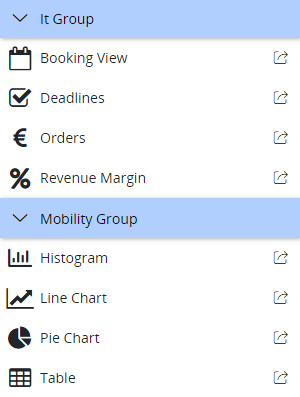
\includegraphics[width=4cm]{Images/lista_widget.png}
  \caption{Lista dei widget realizzati}\label{fig:git}
\end{center}
\end{figure}
\FloatBarrier

\paragraph{Gruppo IT}
\begin{itemize}
    \item Booking view widget: 

\begin{figure}[ht]
\centering
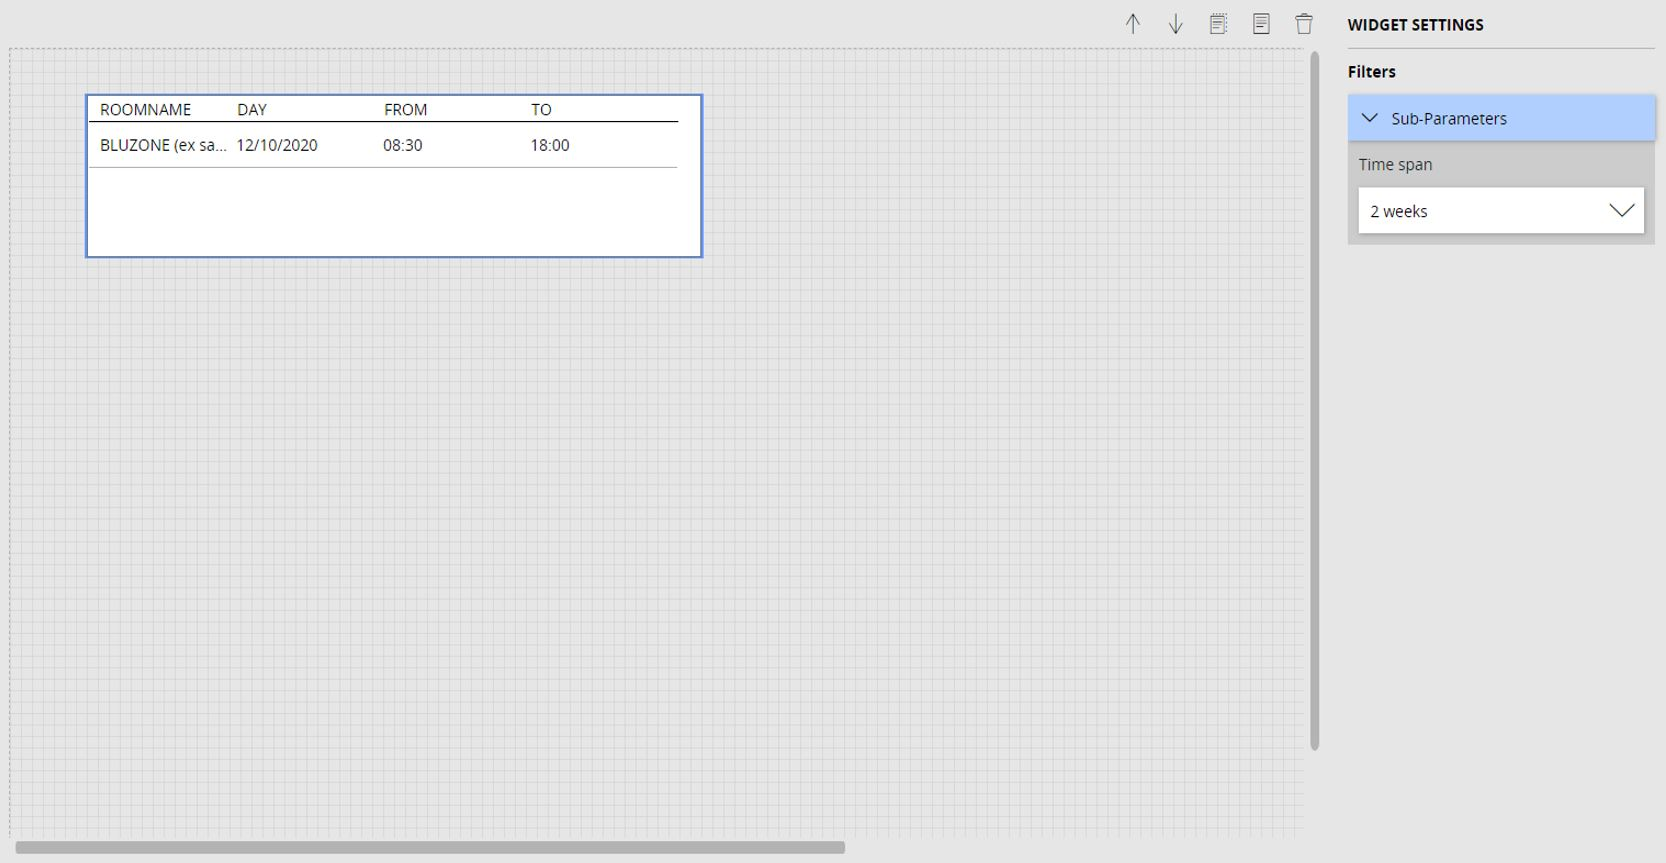
\includegraphics[scale=0.32]{Images/BookingView.JPG}
\end{figure}
permette di visualizzare le prenotazioni dei salottini (stanze predisposte per effettuare riunioni). I parametri sulla destra filtrano i dati secondo l'arco di tempo selezionato, partendo dalla data corrente.
\end{itemize}
\pagebreak
\begin{itemize}
    \item Deadlines widget: 
    
\begin{figure}[ht]
\centering
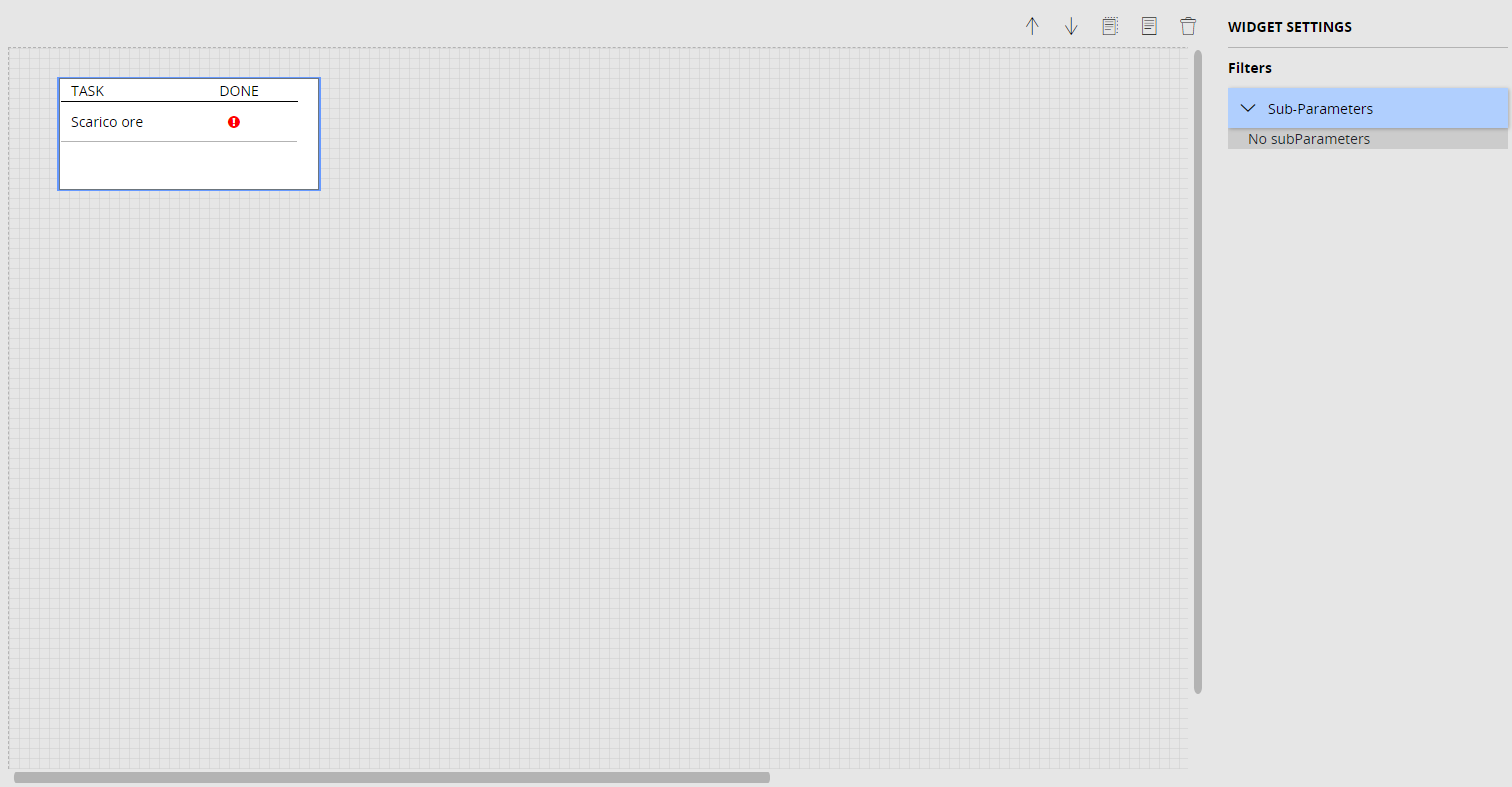
\includegraphics[scale=0.35]{Images/Deadlines.png}
\end{figure}
permette di visualizzare un allarme in base alle scadenze dell'utente autenticato nel sistema.
\end{itemize}
\begin{itemize}
    \item Orders widget: 
    
\begin{figure}[ht]
\centering
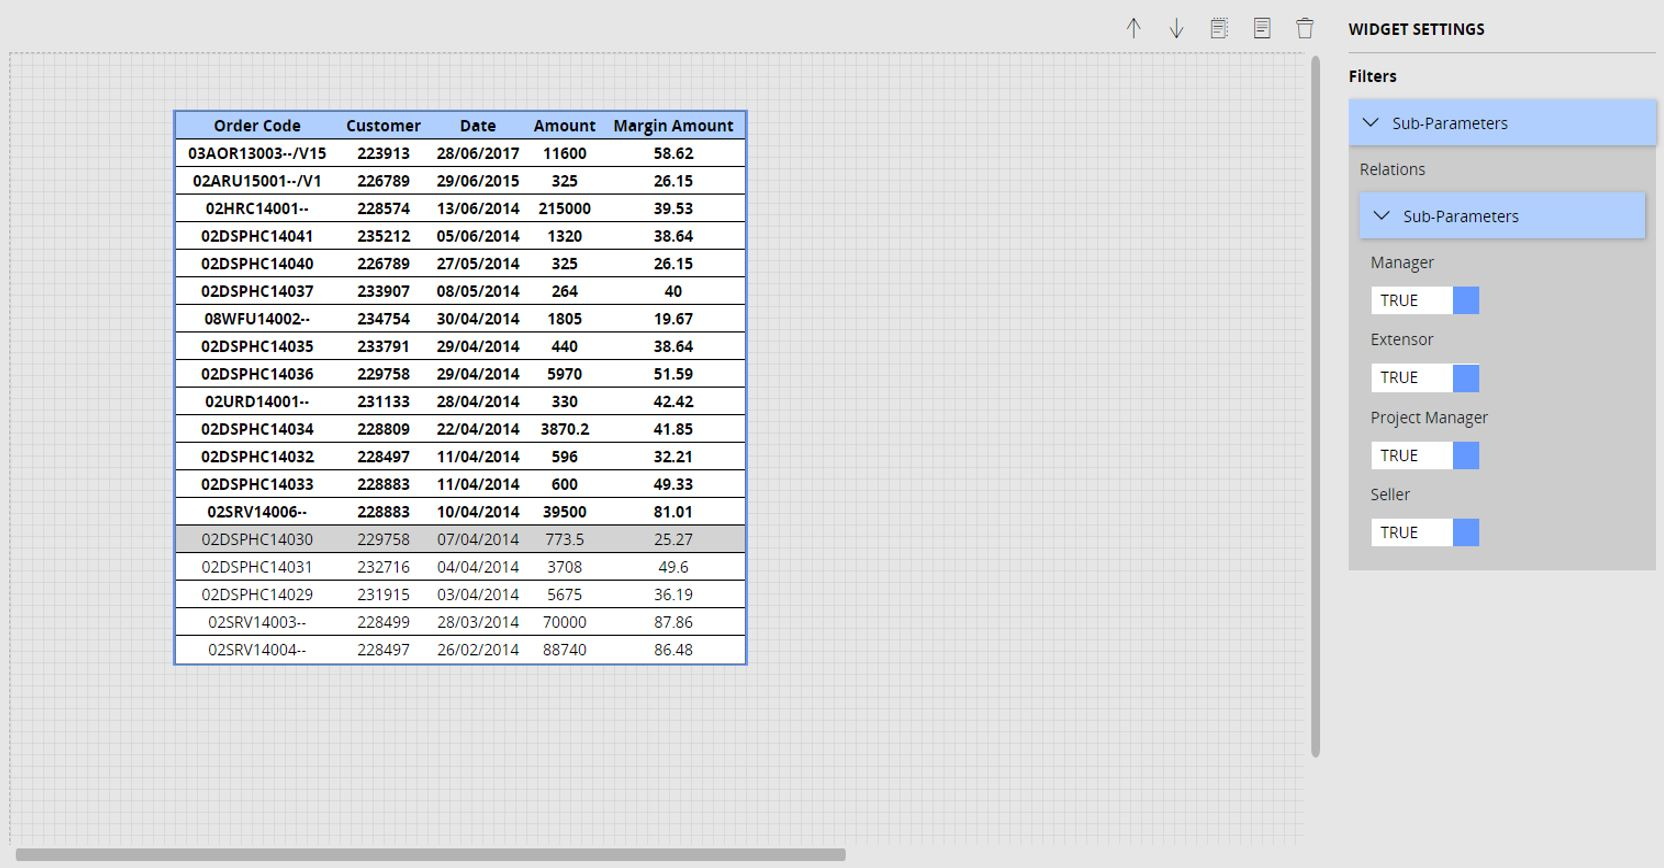
\includegraphics[scale=0.32]{Images/Orders.JPG}
\end{figure}
permette di visualizzare informazioni relative agli ordini. I parametri sulla destra filtrano i dati in base al ruolo che l'utente ricopre per quell'ordine.
\end{itemize}
\pagebreak
\begin{itemize}
    \item Revenue margin widget: 
    
\begin{figure}[ht]
\centering
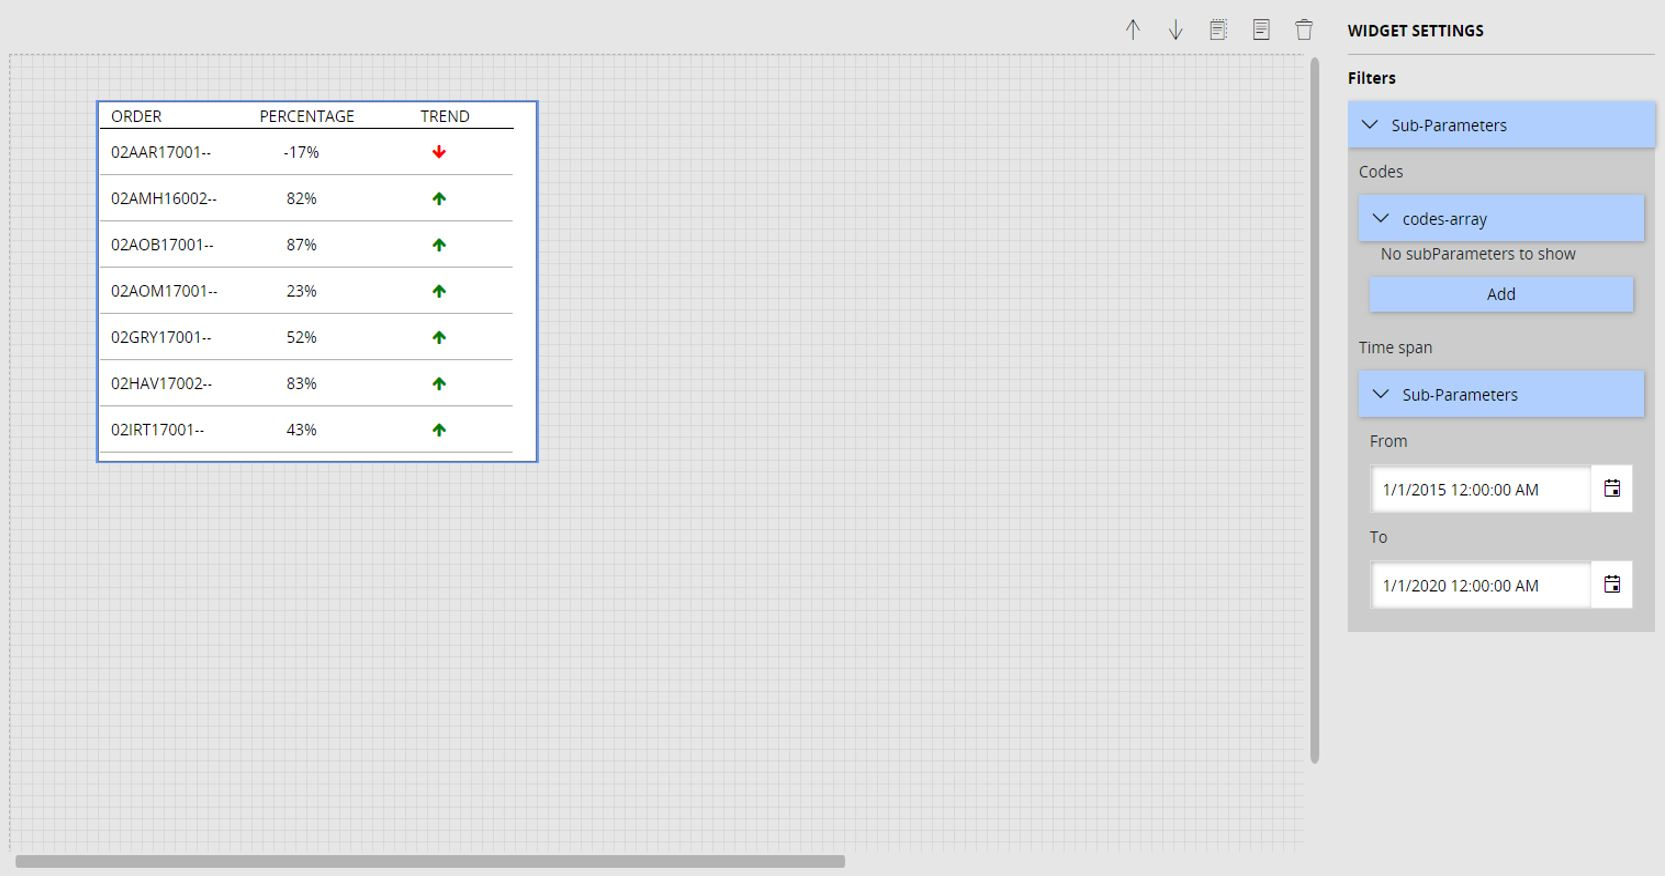
\includegraphics[scale=0.32]{Images/RevenueMargin.JPG}
\end{figure}
permette di visualizzare il trend delle commesse e il valore in percentuale. I parametri sulla destra filtrano i dati in base all'arco di tempo selezionato e permettono di aggiungere ulteriori commesse al widget.
\end{itemize}
% FINE WIDGET IIIIIIIIIIIIIIIIIIT
\paragraph{Gruppo Mobility}
\begin{itemize}
    \item Histogram widget: 
    
\begin{figure}[ht]
\centering
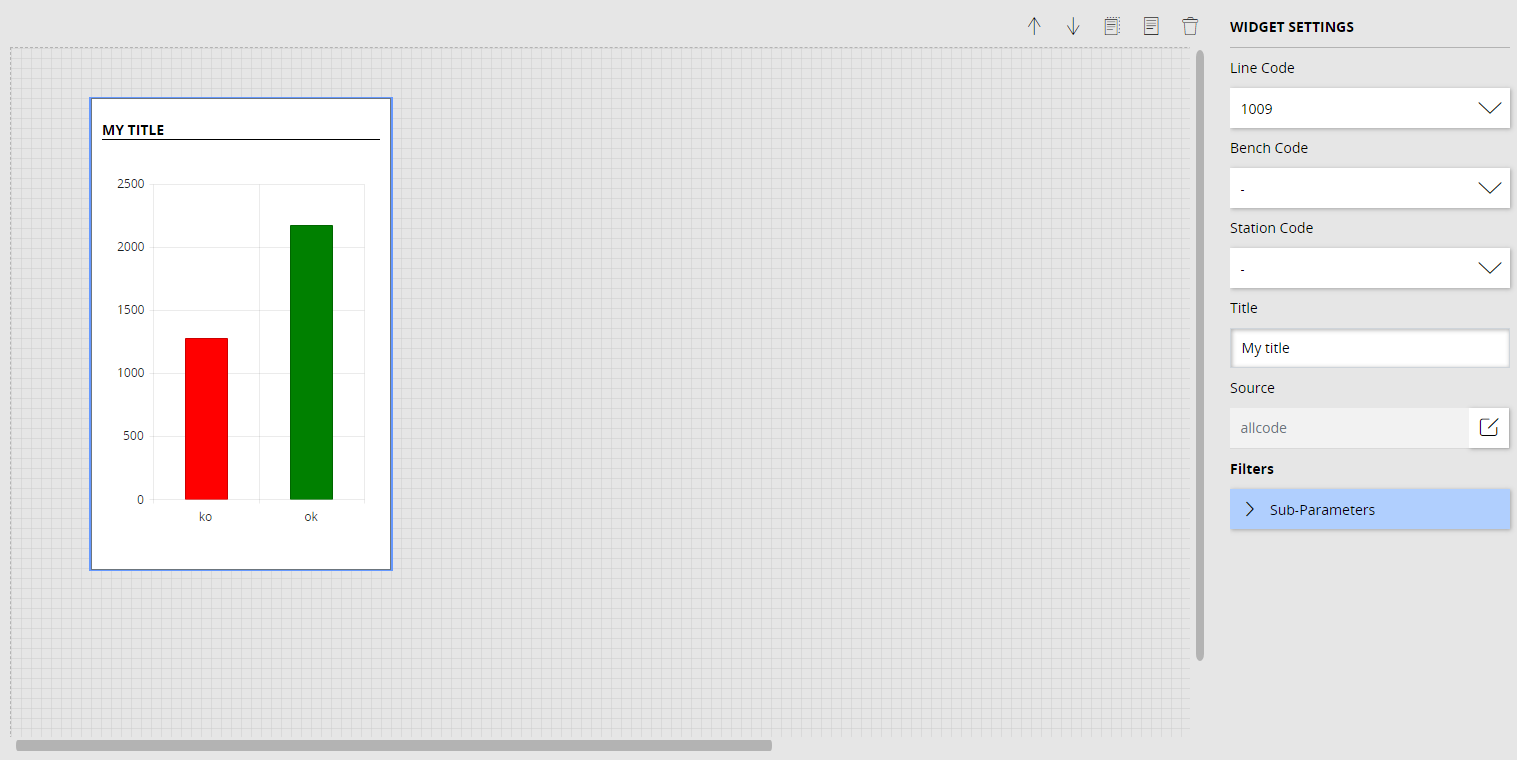
\includegraphics[scale=0.265]{Images/Histogram.png}
\end{figure}
permette di visualizzare dati provenienti dalle macchine Loccioni in un grafico ad istogramma. I parametri sulla destra filtrano i dati e permettono all'utente di selezionare la source da cui prendere i dati.
\end{itemize}
\pagebreak
\begin{itemize}
    \item Pie chart widget: 
    
\begin{figure}[ht]
\centering
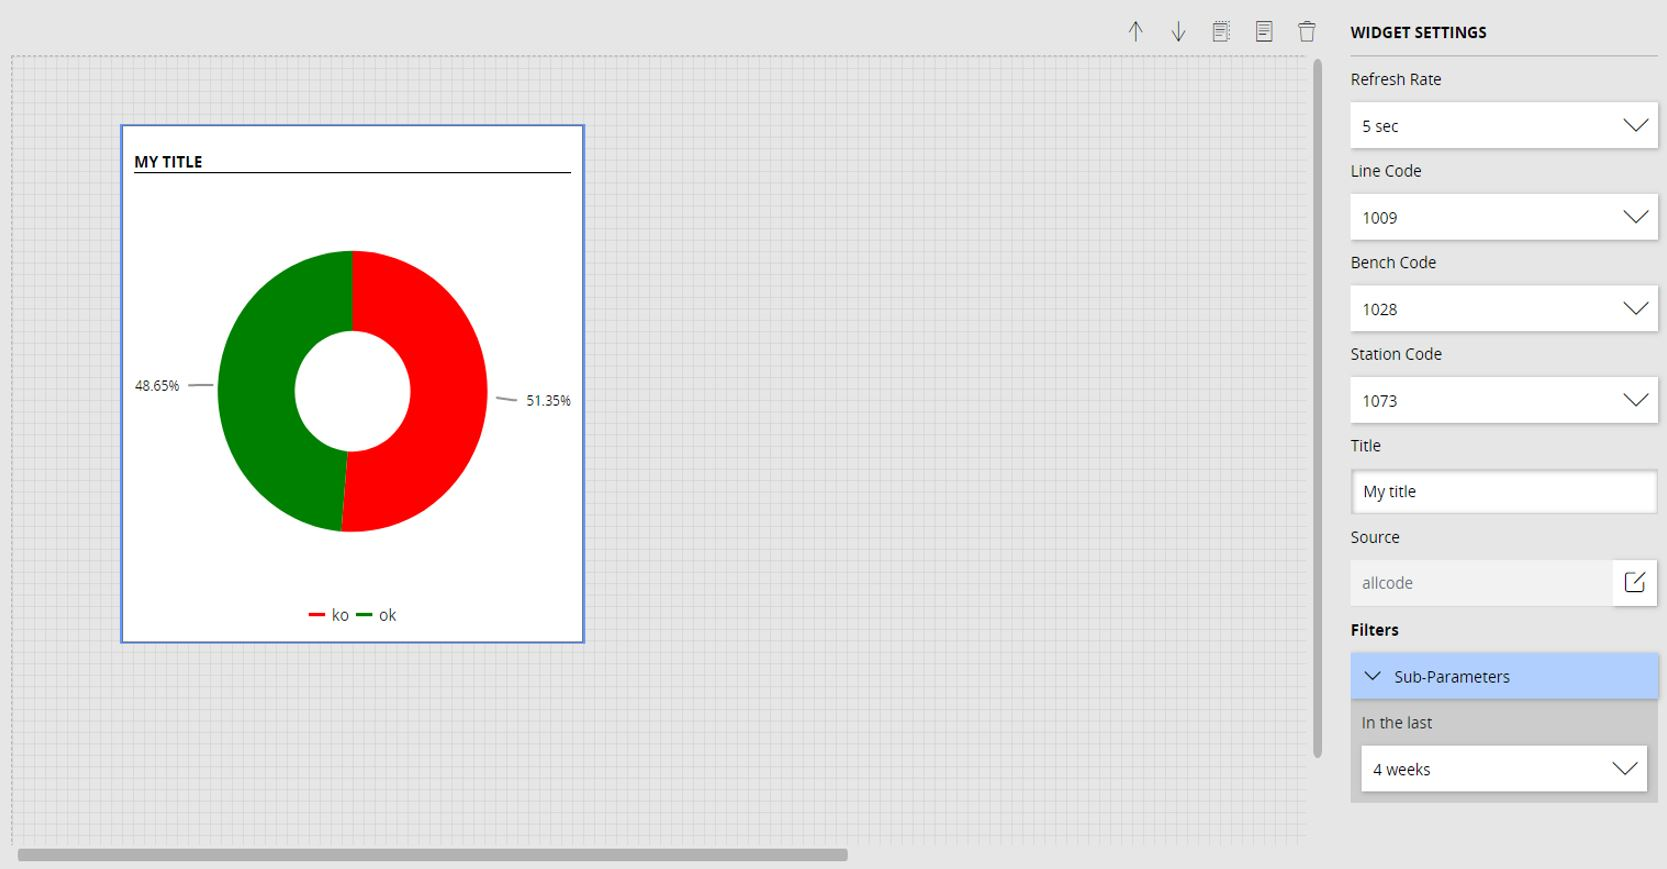
\includegraphics[scale=0.32]{Images/Piechart.JPG}
\end{figure}
permette di visualizzare dati provenienti dalle macchine Loccioni in un grafico a torta. I parametri sulla destra filtrano i dati e permettono all'utente di selezionare la source e di cambiare l'intervallo di tempo in cui il widget ricarica i dati dal backend.
\end{itemize}
\begin{itemize}
    \item Line chart widget: 
    
\begin{figure}[ht]
\centering
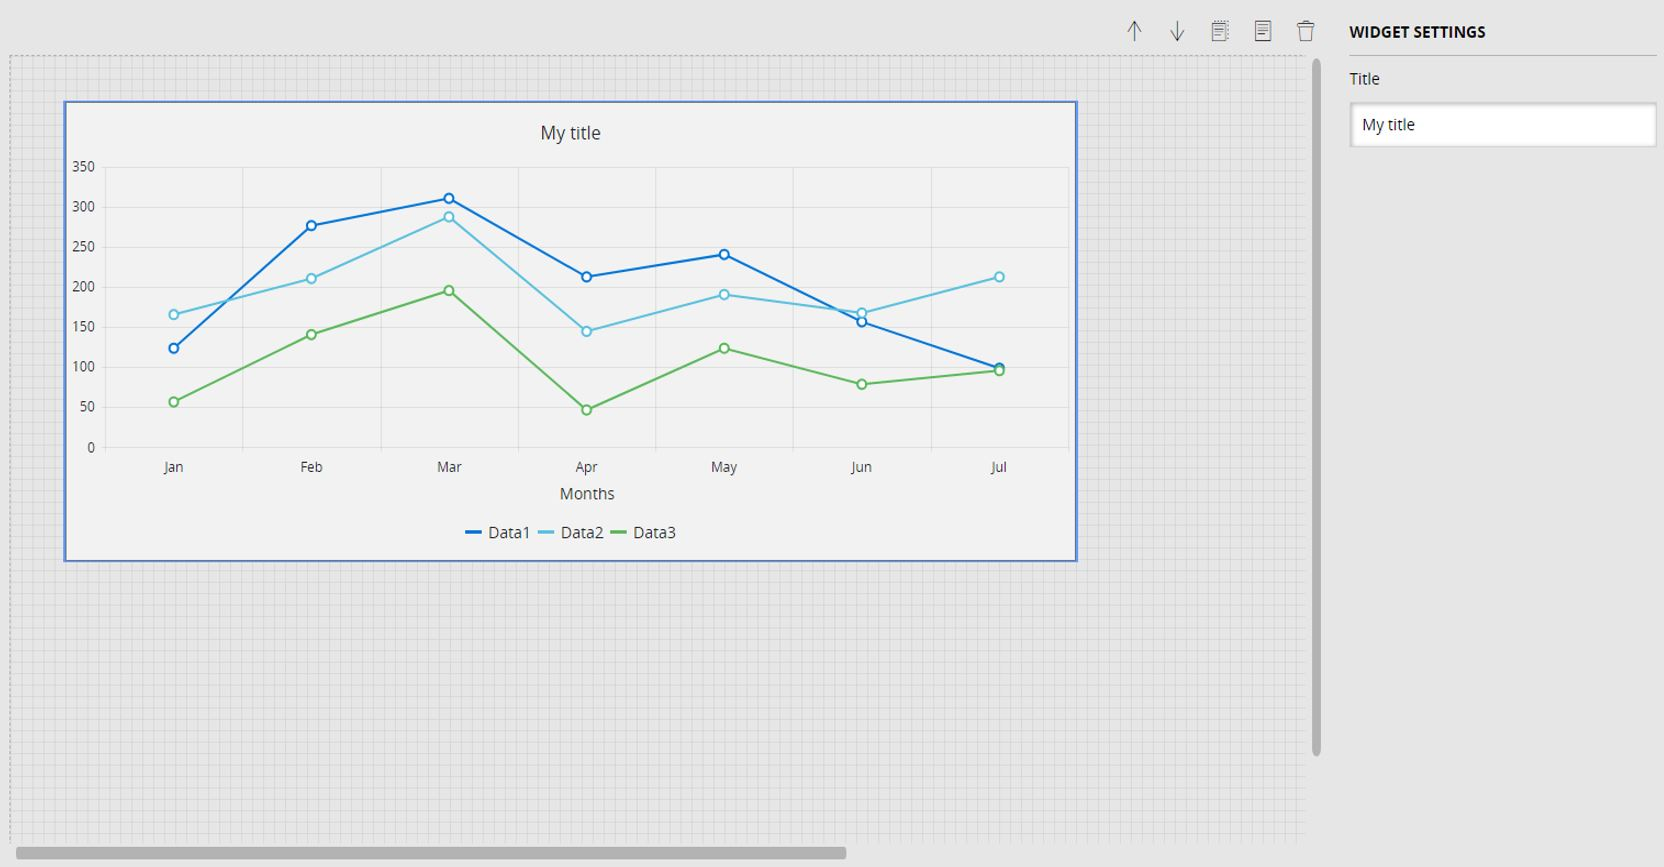
\includegraphics[scale=0.32]{Images/Linechart.JPG}
\end{figure}
permette di visualizzare dati provenienti dalle macchine Loccioni in un grafico a linee.
\end{itemize}

\pagebreak
\begin{itemize}
    \item Table widget: 
    
\begin{figure}[ht]
\centering
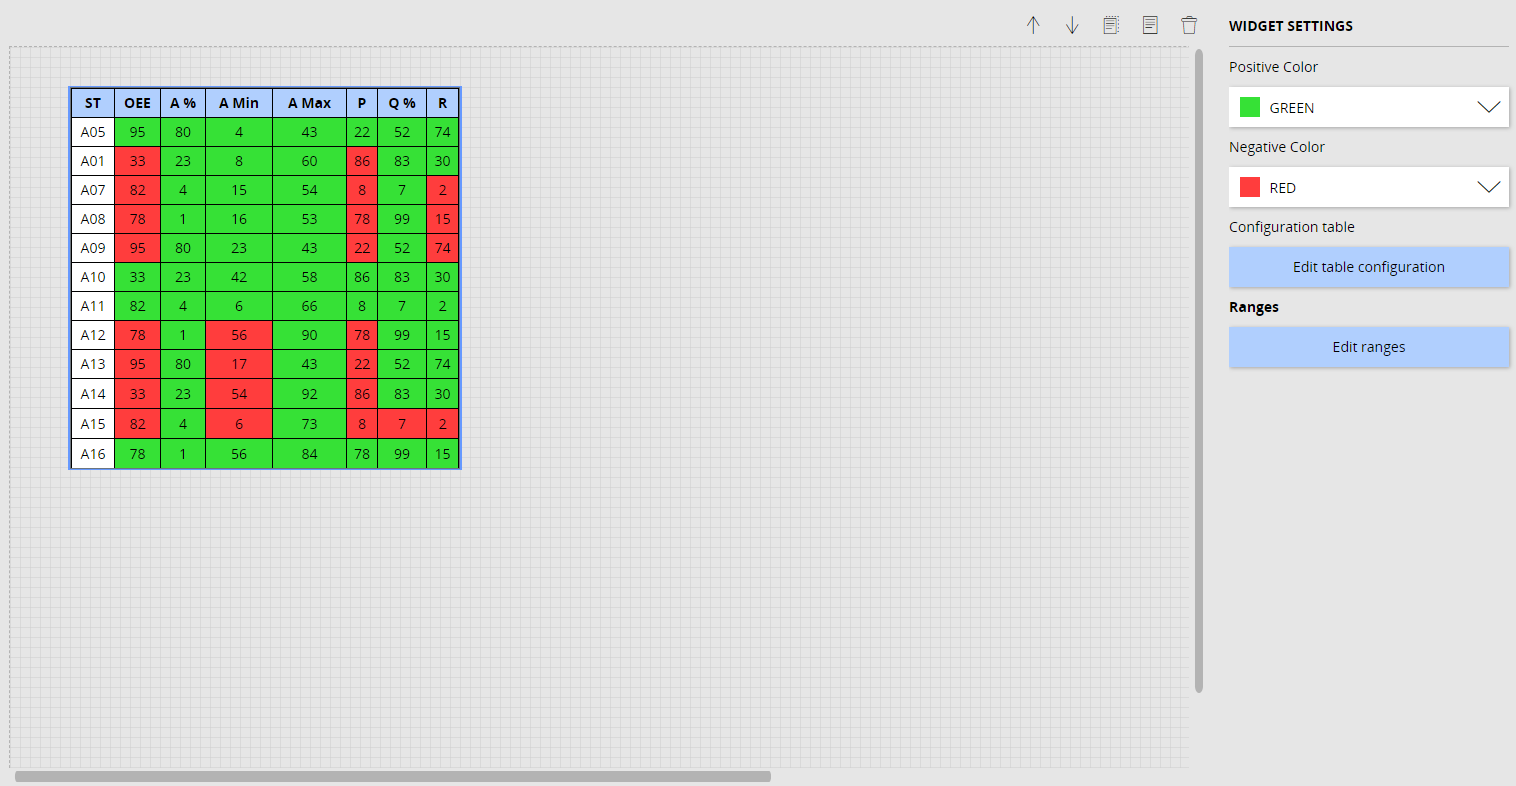
\includegraphics[scale=0.35]{Images/Table.png}
\end{figure}
permette di visualizzare dati provenienti dalle macchine Loccioni in un grafico tabellare. I parametri sulla destra consentono all'utente di specificare le colonne e le righe che si vogliono caricare e consentono di impostare dei range secondo i quali un valore sarà visualizzato come positivo o negativo.
\end{itemize}
Il "line chart widget" ed il "table widget" non sono stati collegati ad alcun database ed utilizzano quindi dati fittizi.




\appendix


\printbibliography


\printindex

%\chapter*{Ringraziamenti}

Ringrazio...

\end{document}
